\documentclass[withoutpreface,bwprint,12pt,a4paper]{cumcmthesis}

\geometry{a4paper, margin=2.5cm}

\usepackage{fancyhdr}

\usepackage{float}

\usepackage[utf8]{inputenc}


\pagestyle{fancy}
\fancyhf{} % 清空页眉页脚设置
\renewcommand{\headrulewidth}{0pt} % 没有页眉线
\fancyfoot[C]{\thepage} % 在页脚中间添加页码

\usepackage{setspace} % 加载设置行距的包
\setstretch{1.25} % 设置1.25倍行距

% 设置标题字体大小和样式
\usepackage{titlesec} % 标题样式包
\titleformat*{\section}{\bfseries\zihao{4}\heiti} % 一级标题:4号黑体
\titleformat*{\subsection}{\bfseries\zihao{-4}\heiti} % 二级标题:小4号黑体 
\titleformat*{\subsubsection}{\bfseries\zihao{-4}\songti} % 二级标题:小4号黑体 


\title{A题:多个火箭残骸的准确定位}
\tihao{A}
\baominghao{4321}
\schoolname{XX大学}
\membera{ a}
\memberb{b }
\memberc{c }
\supervisor{ }%辅导老师
\yearinput{2023}
\monthinput{9}
\dayinput{8}

\begin{document}

\maketitle


 \begin{abstract}%摘要
在现代航天科技领域,火箭是执行太空探索和载荷投放任务的核心设备。鉴于火箭发射活动的高成本和复杂的操作流程,对火箭残骸进行有效的回收与再利用变得至关重要。为了提高火箭残骸的回收效率和精确度,本研究利用已有的实验数据和先进的计算技术,开发了一个高度优化的数学模型,专门用于精确地定位火箭残骸的位置。

该研究首先针对单一火箭残骸的音爆定位问题。具体操作是将地理坐标(经度和纬度)转化为一个适用于高级数学计算的三维坐标系统,包括音爆发生的具体位置(x, y, z 坐标)和发生时间t。本研究应用了三角测量技术来构建相关的数学方程,并通过BFGS(Broyden–Fletcher–Goldfarb–Shanno算法)方法优化了目标函数,即实际音爆与预测音爆时间的差值平方和,以此来精确定位音爆源的确切位置和时间。

接着,研究扩展到多残骸音爆的追踪与定位问题。本模型通过分析各监测站点接收到的音爆数据,确定这些数据分别对应哪一片残骸。为解决这一复杂的多源定位问题,我们建立了一个全新的数学模型,并设定了一个优化目标,即最小化模型预测的音爆到达时间与监测站实际记录时间之间的误差。在这一过程中,模型不仅考虑了时间差、速度和高度限制,还引入了声速随高度变化的约束条件,并且考虑了风速与风向的影响。通过差分进化算法对模型进行非线性最优化处理,最终通过三维可视化技术展示了该模型在实际应用中的有效性,并清晰地展示了监测设备与残骸之间的空间关系。

在误差修正和精准定位的分析阶段,模型考虑到了监测设备记录时间可能包含高达0.5秒的随机误差。通过在每个设备记录的时间中添加一个均值为0,标准差为0.5秒的高斯噪声,我们模拟了现场测量中可能出现的误差。模型的优化目标函数进一步计算了预测音爆抵达时间与观测时间之间的加权平方差,从而在存在随机测量误差的情况下,通过三维可视化及时间分析,对模型结果进行了验证,并展示了模型在估计残骸位置方面的有效性和精确性。

总体来看,通过开发高级数学模型和应用全局优化算法,本研究成功地解决了火箭残骸定位的问题,即使在存在测量误差的情况下,模型也能够提供非常精确的位置估计。这不仅为火箭残骸的回收提供了强有力的技术支持,也为处理类似的复杂定位问题提供了一个有效的求解框架和验证方法。

\keywords{\quad  精确火箭碎片定位\quad 优化模型\quad  差分进化算法\quad 三维可视化技术}
\end{abstract}

%目录  2019 明确不要目录,我觉得这个规定太好了
%\tableofcontents

%\newpage

\section{问题重述}

\subsection{问题背景}
在现代航天任务中,火箭发挥着核心角色。考虑到火箭发射的经济损耗及火箭本身结构复杂性,火箭的残余部分的回收工作变得尤为关键。通常情况下,多级火箭在任务的不同阶段会释放部分如助推器等,这些部件最终会返回地球。这些部件不仅可能重复利用,还可能对地面设施构成潜在风险。因此,快速且准确地定位这些碎片,以便进行回收,是至关重要的。

多级火箭在其任务完成后,通常会通过专门的装置自动解体。这些解体的部分,如助推器和引擎模块,会按照预设轨迹坠向地面。这些部件在穿越大气层时,由于速度超过音速,会引发音爆,此现象源于其高速运动时压缩声波所产生的强烈冲击波。

为了有效地回收这些宝贵的组件,已经开发出一种基于震动波监测的先进定位技术。这项技术涉及在预计的碎片坠落区域布置多个监测站。这些站点能够探测到由超音速飞行的火箭碎片产生的音爆引发的冲击波。通过精确测量这些冲击波在不同监测站的到达时间,可以准确地估算出音爆发生的位置。

该定位系统的核心技术是三角测量法,至少需要三个监测站成功接收到音爆信号。通过分析信号在不同站点到达的时间差异,可以准确锁定音爆的源位置。计算中还需要考虑声速随环境变化的不同而调整,以确保定位的准确性。

确定音爆位置后,利用弹道预测方法估算碎片的潜在落点,这一预测考虑了碎片下落过程中的速度、角度以及地理和气象条件等因素。通过对这些参数进行精确测量与计算,能预测碎片的降落轨迹,从而快速定位其落点。

此外,这种精确的定位技术不仅对碎片回收至关重要,也有助于减少这些碎片对地面造成的潜在损害。通过及时回收这些空间器材,可以大幅度减少发射成本和减轻对环境的影响。

综合来看,随着航天活动的增加,迅速精确地追踪和回收火箭碎片显得尤为关键。这不仅能提高资源的再利用效率,也是确保地面安全和促进航天技术发展的关键。随着监测与回收技术的进步,未来火箭碎片的回收将更加高效和精确。

\subsection{问题回顾}

\subsubsection{问题1单一火箭碎片音爆定位}
构建数学模型,用于精确计算单个火箭碎片在空中产生音爆的具体位置和时间。设定七个监测站点围绕预测的落点,每个站点都记录了音爆到达的时间。探讨如何使用这些数据确定音爆的精确位置和发生时间。

\subsubsection{问题2多碎片音爆监控与定位}
当有多个火箭碎片(如一级火箭主体和几个辅助助推器)同时产生音爆时,各监测站可能会接收到多组不同的冲击波信号。开发数学模型来辨识每个信号对应的碎片,并分析确保所有碎片位置和时间准确确定所需的最小监测站数量。

\subsubsection{问题3复杂多碎片音爆数据分析}
应用问题2中开发的模型,根据监测设备记录的各碎片音爆到达时间,计算每个碎片的精确位置和时间。设备布局及音爆时间间隔假定连续且时间差不超过5秒。

\subsubsection{问题4误差修正与精确音爆定位}
考虑到监测设备记录时间可能包含高达0.5秒的随机误差,调整问题2的模型以更准确地确定各碎片的音爆位置和时间。通过模拟引入随机时间误差的数据来展示修正后模型的效果,并分析其结果误差。讨论若时间误差无法进一步降低的情况下,如何通过模拟监测设备位置和音爆到达时间数据来实现碎片的精确空中定位(误差以公里计)。

\section{问题分析}

\subsection{单个残骸定位分析}

为了解决单个残骸的定位问题,关键步骤是将地理坐标(经度、纬度)转换为笛卡尔坐标系,以简化计算。给定的7个监测设备提供了三维坐标和音爆到达时间,可以利用三边测量技术。通过构建和求解方程组,能够确定音爆发生的位置(x, y, z)和时间(t)。这个过程涉及测量点到音爆点之间的距离与声速和时间差的关系。

\subsection{多个残骸定位分析}

针对多个残骸的定位,需要先识别每个监测设备接收到的音爆数据对应哪个残骸。这是一个优化问题,通过最小化预测音爆位置与实际接收时间之间的误差来确定残骸的准确位置和音爆时间。解决这个问题可能需要非线性优化或迭代重定位技术。

将监测设备的坐标转换到笛卡尔坐标系是空间计算的第一步。每个设备记录了多个音爆时间,必须先确定这些时间点归属于哪个残骸。通过比较设备间音爆抵达时间的差异,并将其与声速计算得出的理论传播时间差进行匹配,可以实现这一点。设定一个优化问题,以确定每个残骸的位置和音爆时间,并最小化预测的音爆抵达时间与实际记录时间之间的误差。

使用梯度下降或牛顿法等非线性优化方法解决每个残骸的位置和音爆时间。由于问题的非线性和可能的多解性,合适的初始估计和约束条件是必要的,以确保解的收敛性和合理性。

\subsection{带有随机误差的定位分析}

针对带有随机误差的定位问题,首先要为每个设备记录的时间引入随机误差,以模拟测量中的不确定性。可以通过添加一个均值为0、标准差为0.5秒的正态分布噪声来实现。面对含随机误差的数据,需要采用更稳健的定位技术,例如加权最小二乘法,其中权重与设备的测量精度相关。

通过改进的模型进行参数优化,求解残骸的位置和时间。噪声的引入可能需要更频繁的迭代或使用更高级的优化算法,以确保达到全局最优解。

\section{模型假设}

为确保所建模型的实际应用性和结果的可靠性,本研究在模型开发前提出了一系列假设。首先,所有使用的数据被假设为真实且有效。其次,认为脱敏处理没有对数据完整性造成负面影响。此外,假定震动波的传播速度为每秒340米。在测算任意两点间的距离时,假设可以忽略地表曲率,具体假设纬度间每度距离为111.263公里,经度间每度距离为97.304公里。这些假设使得模型预测更为合理,同时提升了模型的完整性和实用性。

\section{符号说明}

\begin{table}[H]
    \centering
    \begin{tabular}{ll}
        \toprule % Top line
        符号 & 符号说明 \\
        \midrule % Middle line
        $r_{ij}$ & 简单相关系数 \\
        $\alpha_{ij}$ & 偏相关系数 \\
        $S_{i}$ & 第i个评价对象 \\
        $\mu_{j}$ & 第j个指标的样本均值 \\
        $s_{j}$ & 第j个指标的样本标准差 \\
        $\lambda_j \ (j=1,2,...,9)$ & 特征值 \\
        $b_j$ & 累积贡献率 \\
        $X_{ij}$ & 表示第i个样本第j个指标的数据 \\
        $X$ & 原始样本数据 \\
        $\text{min}(X)$ & 原始样本数据的最小值 \\
        $\text{max}(X)$ & 样本数据的最大值 \\
        \bottomrule % Bottom line
    \end{tabular}
\end{table}


\section{模型的建立与求解}

\subsection{问题一模型的建立与求解}

\subsubsection{数据分析}
利用Python以及所提供的数据资源,制作了以下图形,精确展示了数据的原始位置。这种方法不仅增强了数据的可读性,也方便了对数据位置的直接观察。

\begin{figure}[H]
    \centering
    % 第一张图片
    \begin{minipage}{0.48\textwidth}
        \centering
        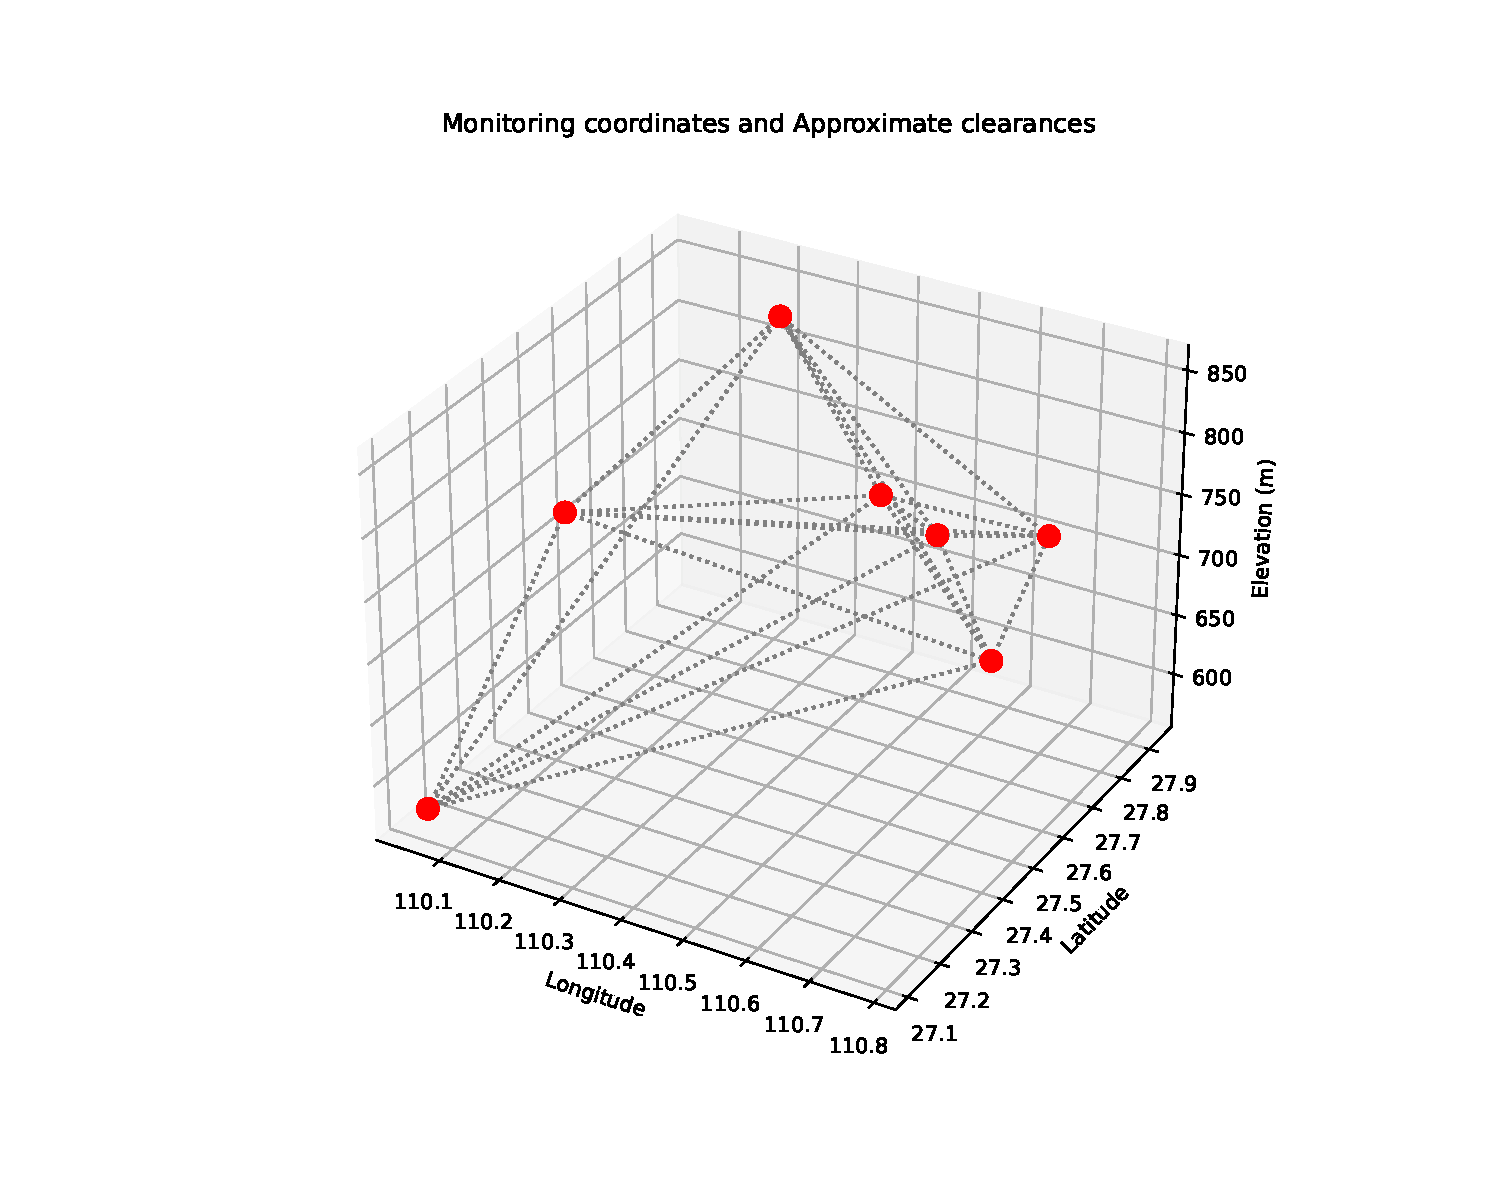
\includegraphics[width=\textwidth]{fig_1}
        \caption{数据的原始位置}
    \end{minipage}\hfill
    % 第二张图片
    \begin{minipage}{0.48\textwidth}
        \centering
        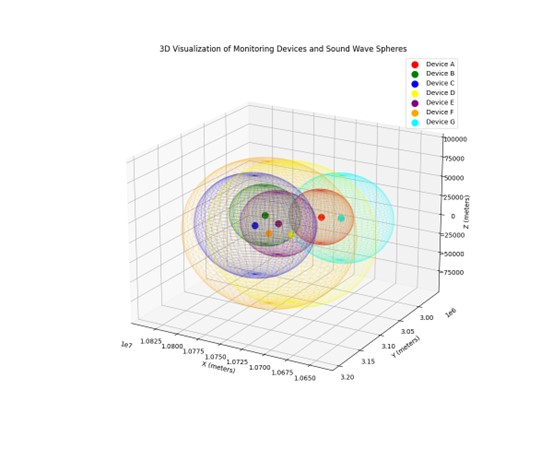
\includegraphics[width=\textwidth]{fig_2}
        \caption{数据的最终位置} % 如果需要第二张图片的标题
    \end{minipage}
\end{figure}


设备A与设备G在该坐标系统中分别处于较高与较低的位置,这表明设备布置考虑了不同的地形高度,通过这种三维配置,设备能有效探测从多个高度和方向传来的音爆信号。此外,图中还详细展示了设备间的相对距离,这一信息对于基于声波传播时间差进行音爆位置分析至关重要。通过构建以监测设备为中心,声波到达时间映射为半径的三维声波传播球体,不同颜色的球体重叠部分清楚地标出了音爆的可能起源位置。这种方法提供了一种直观的方式,以定位并理解音爆事件的空间动态。



\subsubsection{建立单个残骸定位}
首先,将设备的地理位置(经度和纬度)转换到一个更便于进行计算的坐标系统,例如笛卡尔坐标系。转换方法为:X坐标可通过纬度乘以111263米计算(这是纬度一度对应的距离),而Y坐标则由经度乘以97304米得出(这一值根据纬度有所不同)。

\textbf{使用实际米制系统的高程值作为Z坐标}

\begin{table}[H]
    \centering
    \begin{tabular}{lllll} % 修改为5列
        \toprule
        站点 & X (米) & Y (米) & Z (米) & 时间 (秒) \\
        \midrule
        A & 10,726,890.26 & 3,026,798.65 & 824 & 100.767 \\
        B & 10,779,337.12 & 3,054,836.93 & 727 & 112.22 \\
        C & 10,772,720.45 & 3,091,442.46 & 742 & 188.02 \\
        D & 10,727,863.30 & 3,095,892.98 & 850 & 258.985 \\
        \bottomrule
    \end{tabular}
    \caption{站点数据}
    \label{tab:site_data}
\end{table}


残差是每个时间点 \( (x, y, z) \) 到射程 \( t \) 的差异。当提供了各设备的三维坐标和射程数据时,可以使用多项式函数来构建方程组,对每个监测设备i,形成以下方程:

\[ c \dot (t_i - t) = \sqrt{(x - x_i)^2 + (y - y_i)^2 + (z - z_i)^2} \]

其中,\( (x_i, y_i, z_i) \) 及 \( t_i \) 分别代表第i个设备的坐标和时间数据。解决这一方程组是为了得到 \( (x, y, z, t) \) 的值。

为了解四个设备所构成的方程组,至少需要四组数据,即至少需要布置四台监测设备,即可完成后续计算。
本案例中有七台监测设备,允许建立一个优化目标来解决问题,以便预测实际问题中可能出现的偏移。定义一个目标函数,此函数旨在最小化除 \( (x, y, z) \) 位置外的所有误差,并通过寻找最优时间来优化设备间隔。通过运用BFGS方法最小化目标函数,寻找能够表示最终距离估计误差和时间的最小参数值。

目标函数定义为:

\[ f(v) = \sum_{i=1}^L \left[ t + \frac{\sqrt{(x - x_i)^2 + (y - y_i)^2 + (z - z_i)^2}}{c} - t_i \right]^2 \]

其中,
\begin{itemize}
    \item \( v \) 包含位置 \( x, y, z \) 及时间 \( t \) 的向量。
    \item \( t \) 是建模的时间。
    \item \( (x, y, z) \) 是预定目标的坐标位置。
    \item \( c \) 代表速度。
    \item \( (x_i, y_i, z_i) \) 是第i个设备的坐标数据。
    \item \( L \) 代表设备总数。
    \item \( f(v) \) 是预测时间与实际时间之差的平方和。
\end{itemize}


\subsection{事件距离定位的求解}

\subsubsection{最小化过程}
BFGS (Broyden-Fletcher-Goldfarb-Shanno) 算法是用于无约束优化问题的一种迭代方法,它寻求找到函数的局部最小值。以下是该算法在标准定位问题中寻求最小化目标函数时的基本工作原理:

\paragraph{初始化}  
选择一个初始猜测点 \(v_0\)(通常基于第一次测量的坐标和距离数据)并将 Hessian 矩阵的逆初始化为单位矩阵 \(I\)。

\paragraph{迭代步骤}  
在每一次迭代 \(k\) 中,进行以下操作:

\begin{enumerate}
    \item 从当前点 \(v_k\) 的目标函数的梯度 \(\nabla f(v_k)\) 计算出试探步骤方向。
    \item 乘以当前的 Hessian 矩阵的逆近似 \(B_k^{-1}\),以确定前进方向,通常沿负梯度方向进行。
    \[
    p_k = -B_k^{-1} \nabla f(v_k)
    \]
    \item 进行线性搜索以确定最佳步长 \(\alpha_k\),该步长使得目标函数在该方向上达到最小值。
    \[
    \alpha_k = \arg\min_\alpha f(v_k + \alpha p_k)
    \]
    \item 使用确定的步长沿试探方向更新位置。
    \[
    v_{k+1} = v_k + \alpha_k p_k
    \]
    \item 利用新的梯度 \(\nabla f(v_k)\) 更新 Hessian 矩阵的逆近似 \(B_{k+1}\)。
    \item 进行收敛检查:如果位置变化足够小或达到预设的迭代次数,则结束迭代。
\end{enumerate}

\paragraph{输出}  
算法最终输出接近函数局部最小值的参数点 \(v_{k+1}\)。BFGS 算法特别适用于中等规模的优化问题,它不需要计算完整的 Hessian 矩阵,而是利用迭代中收集的信息近似之,从而有效地处理优化问题。在上述定位问题中,BFGS 通过合适的初始猜测并通过多次梯度下降及梯度方向的更新来优化位置和时间的确定。最终输出通常位于最小值的近似区域内。


\textbf{为直观展示结果,使用 Python 绘制的可视化结果如下:}

\begin{figure}[!htbp]
    \centering
    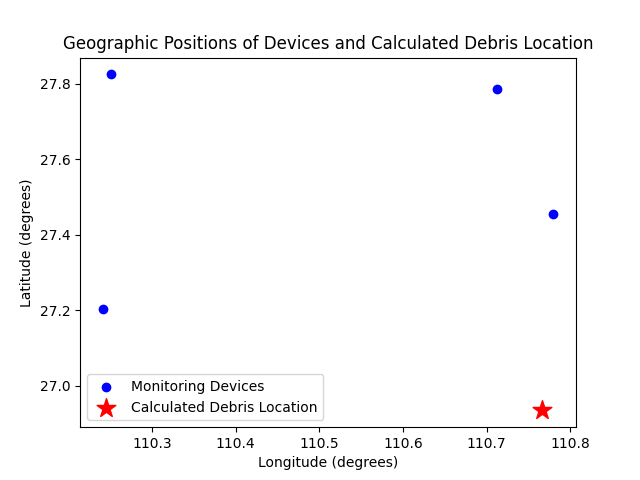
\includegraphics[width=.6\textwidth]{fg3}
	    \caption{} % 添加标题(如有需要)
\end{figure}

\begin{figure}[H]
    \centering
    % 第一张图片
    \begin{minipage}{0.48\textwidth}
        \centering
        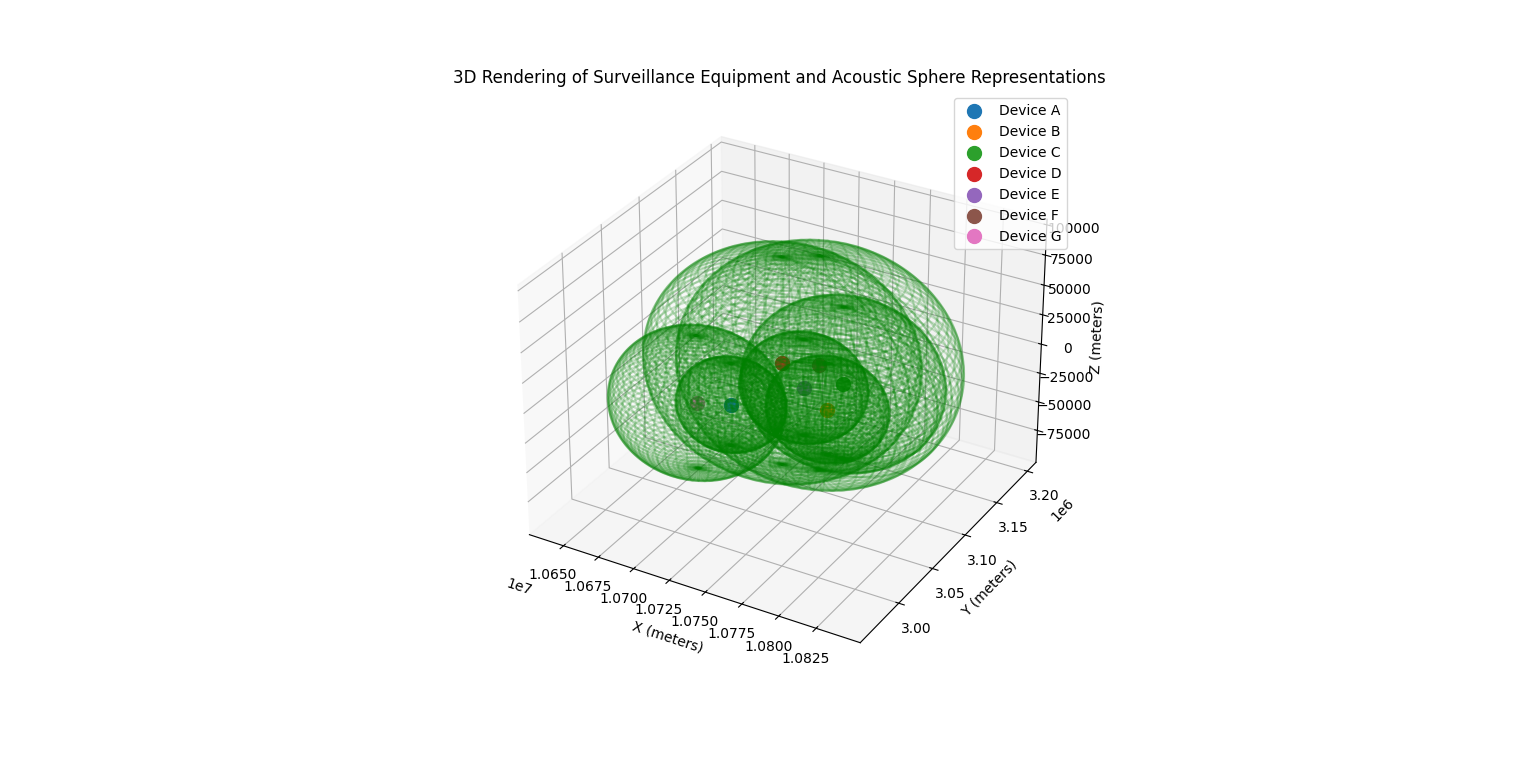
\includegraphics[width=\textwidth]{fig_4}
        \caption{} % 添加标题(如有需要)
        \label{fig:4} % 添加引用标签(如有需要)
    \end{minipage}
    \hfill % 在两个 minipage 之间添加一些空间
    % 第二张图片
    \begin{minipage}{0.48\textwidth}
        \centering
        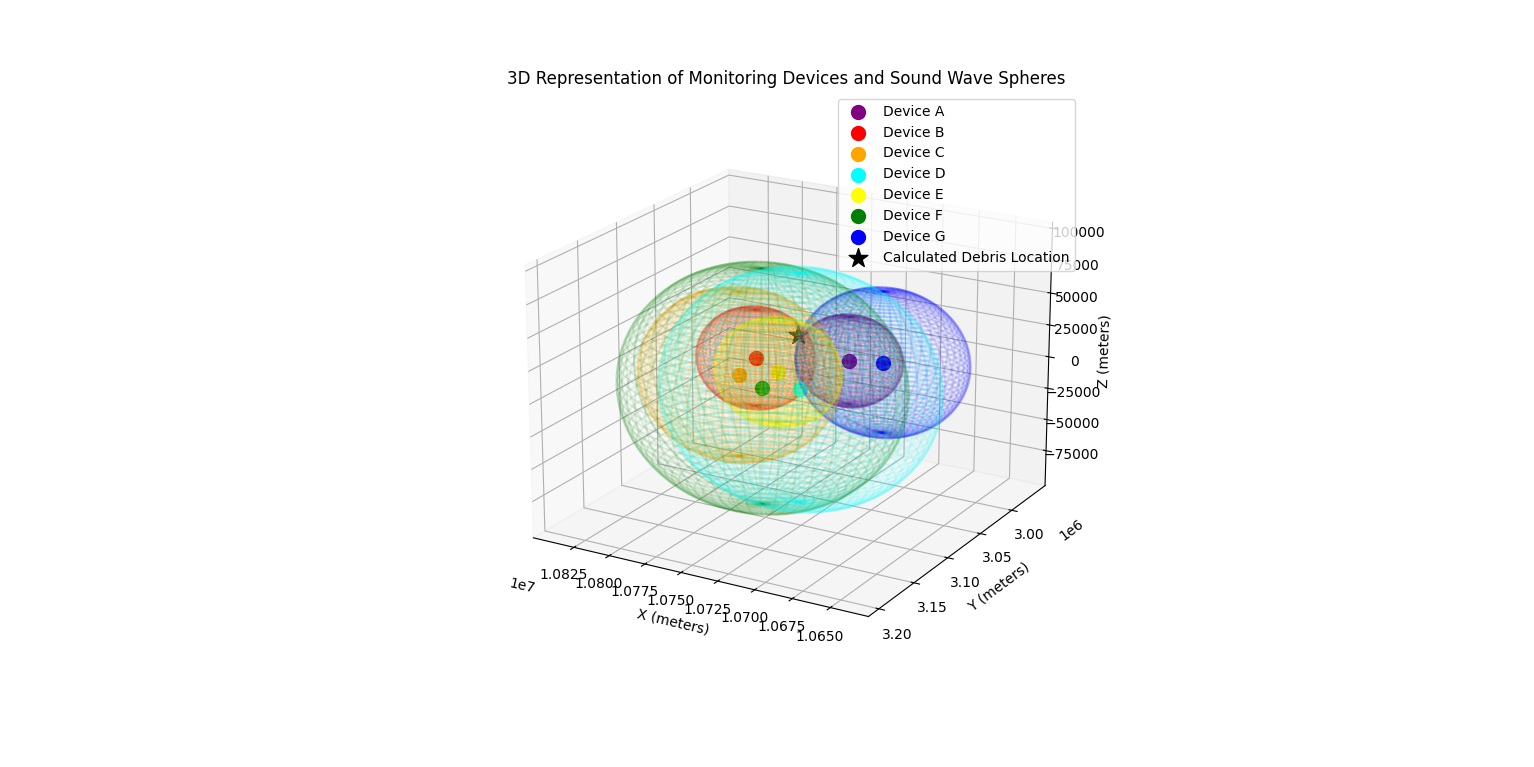
\includegraphics[width=\textwidth]{fig_3}
        \caption{} % 添加标题(如有需要)
        \label{fig:3} % 添加引用标签(如有需要)
    \end{minipage}
\end{figure}



\textbf{最终输出结果如下,其中偏移时间为相对于设备A的记录时间。}


\begin{table}[ht]
\centering % 使用centering命令来居中表格
\begin{tabular}{cccc}
\toprule
参数名称 & 数值 & 单位 \\
\midrule
X坐标 & \(1.07784 \times 10^7\) & 米 \\
Y坐标 & \(2.99621 \times 10^6\) & 米 \\
距离 & 717.63 & 米 \\
偏移时间 & -74.52 & 秒 \\
\bottomrule
\end{tabular}
\end{table}



\subsubsection{问题二三模型的建立与求解}

\paragraph{数据分析}

数据分析表明,声波从音爆源至监测设备的传播可以视为球面波,随着时间推移,这些波的半径不断增大。每当残骸在空中产生音爆时,便会形成一个扩展的声波球。为了更直观地呈现这些现象,本文首先以监测点A为例,在二维和三维平面上绘制了声波球的扩散过程。此方法有助于更深入理解声波的传播和扩散机制。

\begin{figure}[ht]
    \centering
    % 第一排第一张图片

    \begin{minipage}[c]{0.45\textwidth}
        \centering
        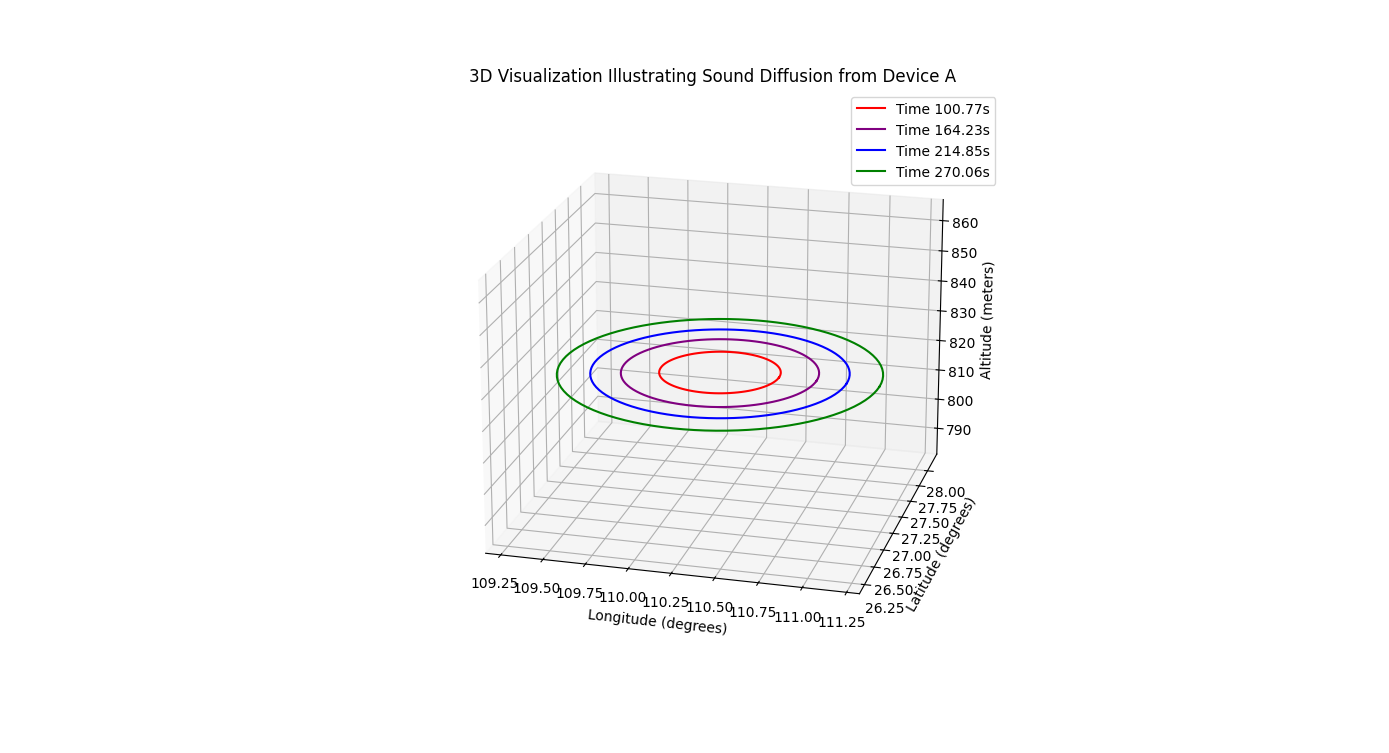
\includegraphics[width=0.95\textwidth]{fig_5}
        \subcaption{} % 你可以添加子标题
        \label{fig:5}  % 你可以添加引用标签
    \end{minipage}
    \hfill % 添加空白填充以对齐图片
    % 第一排第二张图片
    \begin{minipage}[c]{0.45\textwidth}
        \centering
        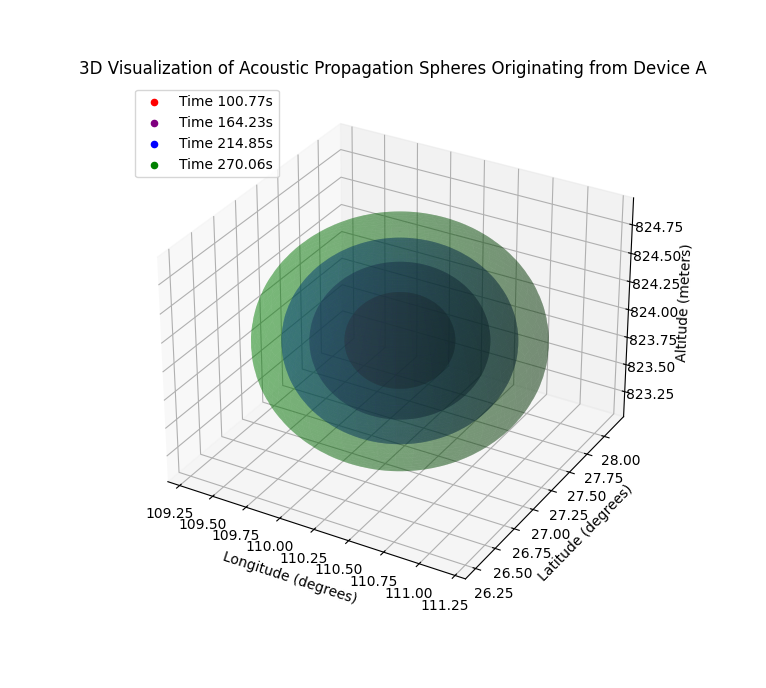
\includegraphics[width=0.95\textwidth]{fig_6}
        \subcaption{}
        \label{fig:6}
    \end{minipage}
    
    % 第二排第一张图片
    \begin{minipage}[c]{0.45\textwidth}
        \centering
        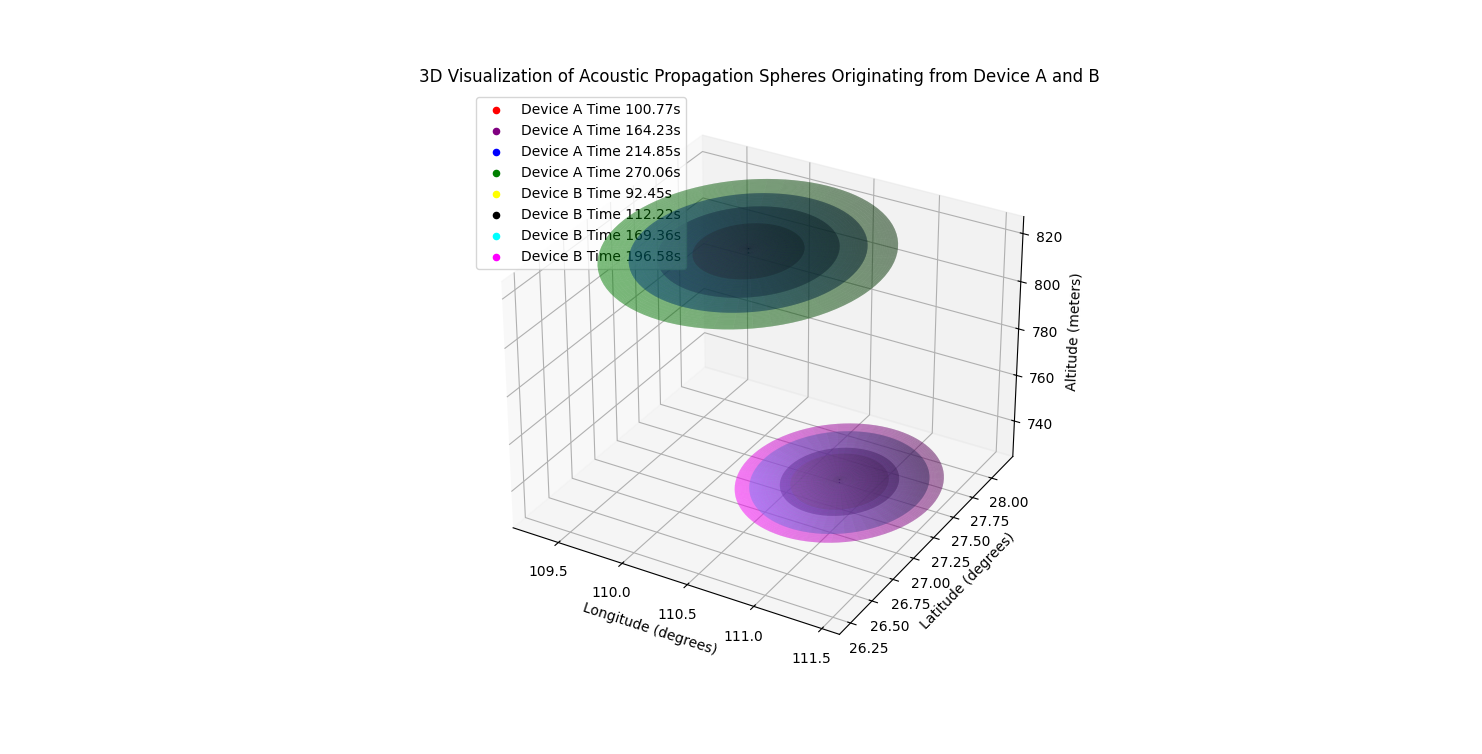
\includegraphics[width=0.95\textwidth]{fig_7}
        \subcaption{}
        \label{fig:7}
    \end{minipage}
    \hfill % 添加空白填充以对齐图片
    % 第二排第二张图片
    \begin{minipage}[c]{0.45\textwidth}
        \centering
        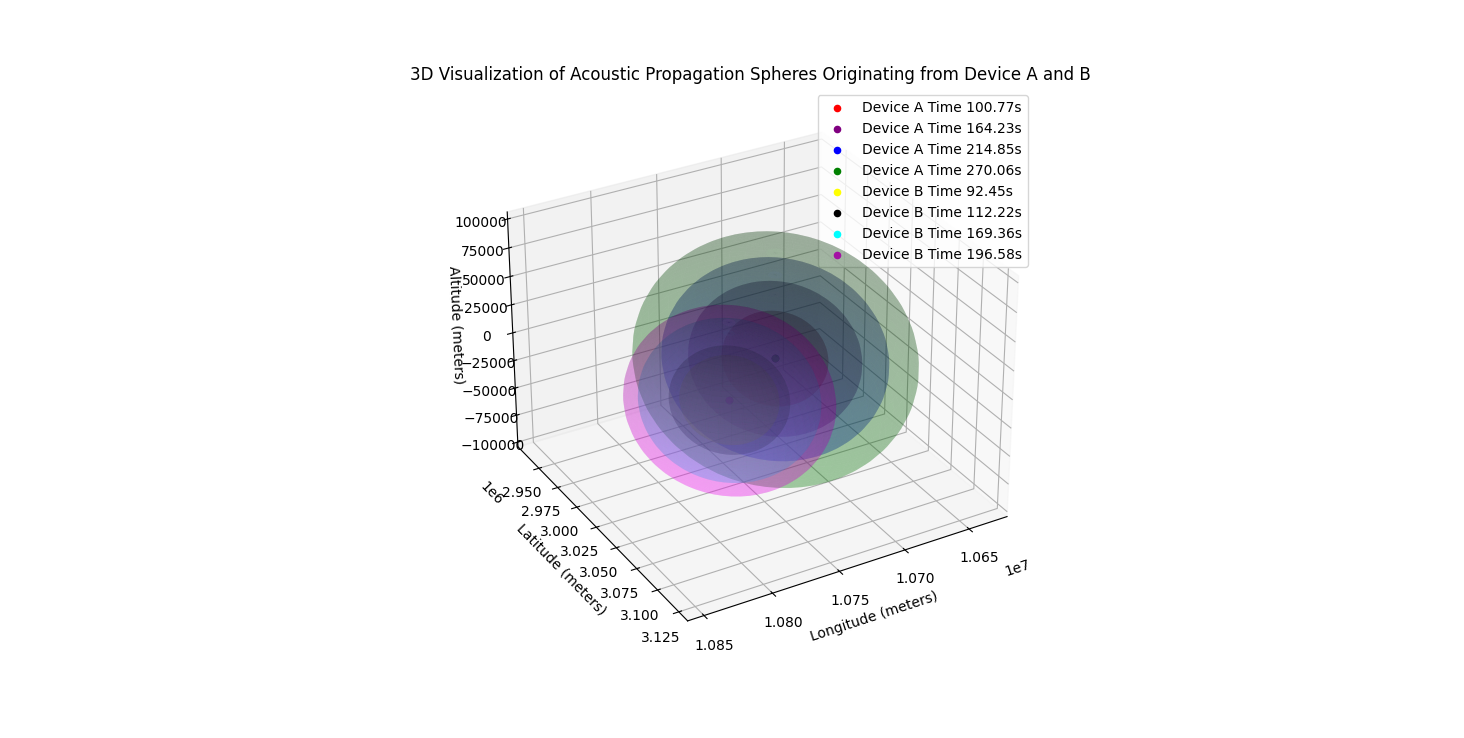
\includegraphics[width=0.95\textwidth]{fig_8}
        \subcaption{}
        \label{fig:8}
    \end{minipage}
	\caption{} % 添加标题(如有需要)
\end{figure}

\paragraph{多个残骸定位模型的建立}

当火箭残骸在空中发生音爆时,会产生一个随时间向外扩散的球形声波。利用多边测量原理,可以根据不同监测站记录到的声波到达时间,定位每个音爆源的确切位置。通过比较来自不同监测站的声波到达时间,采用时间差定位(TDOA)方法,可以精确确定每个残骸的位置。

为了在三维空间中准确确定一个点的位置,至少需要从四个不同的监测站进行数据测量。由于存在四个残骸,至少需要五个监测站才能确保得到一个唯一的解集。这种情况下,通常会采用非线性最小化算法来解决涉及多个变量的优化问题,从而找到所有残骸的最可能的位置和发生时间。

时间差定位是一种基于时间测量确定信号源位置的技术。在此技术应用的情景中,音爆源作为信号源,声波会从该点向外以声速传播。由于各监测站与音爆源的距离不同,它们接收到声波的时间也会不同。因此,每个监测站能够提供一个时间测量值,该值与其到音爆源的距离成正比。

通过至少三个这样的时间测量,可以构建一个求解音爆源位置的方程组。这些方程是关于音爆源位置的非线性方程,涉及未知数的平方及其开方运算。解决这一方程组通常通过数值方法实现,如最小二乘法,因为可能不存在解析解或者解析解难以求得。通过最小化方程的误差平方和,可通过数值优化方法求解这一问题。

在多个音爆源,例如多个火箭残骸的情况下,每个残骸都会产生一个类似的方程组。必须同时解决所有方程组并考虑它们之间的相互关系,这样才能确定每个残骸的位置和音爆时间。这种复杂的情况通常需要更高级的数值算法,并可能涉及到多变量及多目标优化问题的处理。

\paragraph{最终模型说明}

考虑到监测设备的地理位置(经度、纬度、高度)以及它们记录的各测量者设备使用时间(标记为 \(i\) 发射者,\(j\) 为接收者),目标是准确确定每个测量者的三维位置(\(x_i, y_i, z_i\))及信号发送时间 \(T_j\)。

问题设定中的常数 \(c\) 表示光速。设备的地理位置被转换为坐标系中的点 \((x, y, z)_i\)。因此,目标函数定义为所有预测时间与实际时间差的平方和:
\[
f(v) = \sum_{i=1}^n \sum_{j=1}^n \left[ T + \frac{\sqrt{(x-x_i)^2 + (y-y_i)^2 + (z-z_i)^2}}{c} - t_{ij} \right]^2
\]

其中:
\begin{itemize}
    \item \(v\) 是包含 \(x, y, z, t\) 的向量。
    \item \(T\) 是模型建立时间。
    \item \((x, y, z)\) 代表目标坐标位置。
    \item \(c\) 是速度,通常是光速。
    \item \((x_i, y_i, z_i, t_i)\) 分别是第 \(i\) 个设备的坐标和测量时间。
    \item \(n\) 是设备的总数。
    \item 主要目标是最小化 \(f(v)\),即预测时间与实际时间的平方差和。
\end{itemize}

\subparagraph{时间差约束}

重要的一点是所有定位设备的测量时间差不能超过5秒。在目标函数中,对于超过5秒的时间差,引入一个权重惩罚项:
\[
|T_r - T_s| > 5 \, \text{s}, \quad \text{增加目标函数惩罚项}
\]

\subparagraph{速度约束}

考虑到监测的物体(如火箭残骸)可能的最大速度 \(v_{\text{max}}\),每个定位器的位置变化速度不应超过这一最大值:
\[
\sqrt{\left(\frac{dx_j}{dt}\right)^2 + \left(\frac{dy_j}{dt}\right)^2 + \left(\frac{dz_j}{dt}\right)^2} \leq v_{\text{max}}
\]

\subparagraph{高度约束}

设定一个预定的高度范围 \([{\text{min}}, {\text{max}}]\)。每个定位器的高度必须满足:
\[
z_{\text{min}} \leq z \leq z_{\text{max}}
\]

这确保了解决方案符合预期的轨迹。

\subparagraph{声速随高度变化模型}

声速 \(c\) 根据高度变化会有所不同。可以引入一个随高度变化的声速模型 \(c(z)\),以提高时间估算的准确性:
\[
t_{ij} = T_j + \int_{\text{path}} \frac{ds}{c(z)}
\]
其中,积分沿从残骸 \(j\) 到监测站 \(i\) 的路径计算,\(ds\) 是路径元素,\(c(z)\) 是路径上某点的声速。

\subparagraph{风速及风向影响}

考虑风速(\(V_{\text{wind}}\))和风向对声波传播的影响,实际声波传播时间 \(t_{ij}\) 应考虑风的作用:
\[
t_{ij} = T_j + \int_{\text{path}} \frac{ds}{c(z) + \vec{V}_{\text{wind}} \cdot \vec{u}_{ij}}
\]
其中,\(\vec{u}_{ij}\) 为从测量点指向测量点的单位向量,方程表示风向和速度的影响。

\paragraph{模型的最终形式}

\[
\min f(v) = \sum_{i=1}^n \sum_{j=1}^n \left[ T + \frac{\sqrt{(x-x_i)^2 + (y-y_i)^2 + (z-z_i)^2}}{c} - t_{ij} \right]^2
\]
包括如下约束条件:
\begin{itemize}
    \item 时间差约束: \(|T_i - T_j| > 5s\),应用惩罚项。
    \item 速度约束:
    \[
    \sqrt{\left(\frac{dx_j}{dt}\right)^2 + \left(\frac{dy_j}{dt}\right)^2 + \left(\frac{dz_j}{dt}\right)^2} \leq v_{\text{max}}
    \]
    \item 高度约束:
    \[
    z_{\text{min}} \leq z \leq z_{\text{max}}
    \]
    \item 时间计算调整,包括声速及风速影响:
    \[
    t_{ij} = T_j + \int_{\text{path}} \frac{ds}{c(z) + \vec{V}_{\text{wind}} \cdot \vec{u}_{ij}}
    \]
\end{itemize}

\subsection{模型的求解}

差分进化算法(Differential Evolution, DE)是一个高效的全局优化方法,常用于处理各类参数优化难题。该算法基于群体的演化过程,通过交叉、变异和选择操作寻找全局最优解。以下是差分进化算法的标准操作流程:

\begin{itemize}
    \item \textbf{初始化}\\
    随机生成初始种群,每个种群个体(向量)代表一个潜在的解决方案。设定初始控制参数:变异因子(\(F\))、交叉率(\(CR\))和种群规模(\(NP\))。
    
    \item \textbf{变异}\\
    对于每个种群个体 \(x_i\),选择三个不同且与 \(x_i\) 不相同的个体 \(x_a, x_b, x_c\)。
    生成变异向量 \(v_i\) 如下:
    \[
    v_i = x_a + F \cdot (x_b - x_c)
    \]
    其中 \(F\) 是正的缩放因子,调控变异强度。

    \item \textbf{交叉}\\
    通过交叉操作生成候选解向量 \(u_i\),对每个基因位置 \(j\):
    \[
    u_{ij} = 
    \begin{cases} 
    v_{ij} & \text{if } \text{rand}(j) \leq CR \text{ or } j = \text{rand}(1, D) \\
    x_{ij} & \text{otherwise}
    \end{cases}
    \]
    其中 \(\text{rand}(j)\) 是在 [0, 1] 上的随机数,\(CR\) 是交叉概率,\(D\) 是向量维度,确保至少一个基因来自变异向量。

    \item \textbf{选择}\\
    使用贪心策略评估每个个体,如果试验向量 \(u_i\) 的适应度优于当前个体,则替换当前个体以形成新一代。
    \[
    x_i^{t+1} = 
    \begin{cases} 
    u_i & \text{if } f(u_i) \leq f(x_i) \\
    x_i & \text{otherwise}
    \end{cases}
    \]

    \item \textbf{迭代}\\
    重复变异、交叉和选择过程,直到满足结束条件(如达到最大迭代次数、适应度阈值或解的改进停滞)。
\end{itemize}

算法参数设置如下:最大迭代次数为 10000,种群规模为 20,容忍度设置为 0.1。变异因子范围设定在 (0.5, 1),交叉概率为 0.8。

\textbf{最终输出}

通过算法优化后,结果表明四块残骸分布于三维空间的不同区域,每块残骸的具体位置由相应的经度、纬度和高度确定。其中一块残骸明显高于其他,显示出独特的飞行或解体模式。所有残骸的定位时间与模型设定的时间差不超过5秒的约束相符。

经过优化算法处理后,得出的四块残骸的位置分散在三维空间的不同点上,每一块残骸的位置都是由对应的经度、纬度和高度决定的。残骸的高度差异不同残骸的高度差异显著,尤其是残骸4显示了一个远高于其他残骸的高度值(接近9500米),可能指示了不同的飞行轨迹或解体模式。时间结果所有残骸的时间都接近95.77秒,除了残骸4,其时间为99.00秒。这与模型中残骸音爆时间差不超过5秒的约束相符合。

\begin{table}[H]
    \centering
    \begin{tabular}{lllll}
        \toprule
        \textbf{碎片编号} & \textbf{经度} & \textbf{纬度} & \textbf{高度 (米)} & \textbf{时间 (秒)} \\
        \midrule
        1 & 110.460487 & 27.08216 & 836.6 & 95.77 \\
        2 & 110.488886 & 27.65688 & 675.6 & 95.77 \\
        3 & 110.476655 & 27.684826 & 1447.0 & 95.77 \\
        4 & 110.490609 & 29.940262 & 494.3 & 99.00 \\
        \bottomrule
    \end{tabular}
    \caption{碎片数据}
    \label{tab:fragment_data}
\end{table}


通过此优化,生成了三维可视化图,直观显示了各残骸与监测设备之间的空间关系。这些信息对于实地回收工作至关重要,为回收团队提供了精确的定位数据。
\begin{figure}[H]
    \centering
    % 第一张图片
    \begin{minipage}{0.48\textwidth}
        \centering
        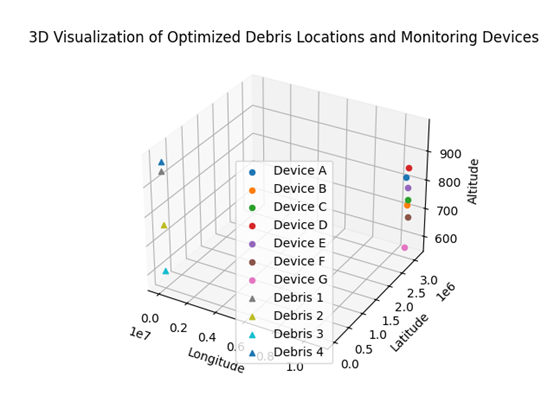
\includegraphics[width=\textwidth]{fig_9}
        \caption{} % 添加标题(如有需要)
        \label{fig:4} % 添加引用标签(如有需要)
    \end{minipage}
    \hfill % 在两个 minipage 之间添加一些空间
    % 第二张图片
    \begin{minipage}{0.5\textwidth}
        \centering
        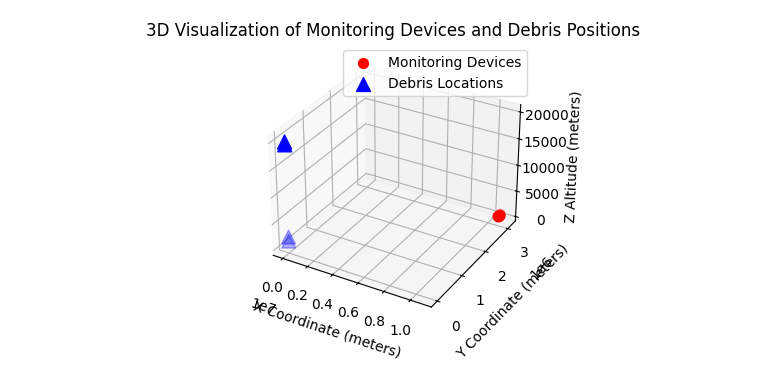
\includegraphics[width=\textwidth]{fig_10}
        \caption{} % 添加标题(如有需要)
        \label{fig:3} % 添加引用标签(如有需要)
    \end{minipage}
\end{figure}

\subsection{问题四模型的建立与求解}

对于同源四维定位,考虑时间记录中存在的随机误差是关键,以便精确确定四个传感器的位置和时间。首先,传播误差随传感器的坐标和时间扩展而增加的不确定性是内在的。每个设备记录时间的随机误差由误差模型进行假设,认为这些误差符合正态分布 \(N(0, \sigma^2)\)。

\[
t_{ij}^{obs} = t_{ij} + \epsilon_i
\]

这里,\(t_{ij}^{obs}\) 是第 \(i\) 个设备在第 \(j\) 次观测到的时间,\( \epsilon_i \) 是附加的随机噪声,其方差 \(\sigma^2\),我们这里设置为 0.5 秒。

目标函数 \(f(v)\) 的目标是最小化时间和空间间隔偏差的平方和,具体表达式如下:

\[
f(v) = \sum_{i=1}^n \sum_{j=1}^n \left[ \frac{t + \sqrt{(x-x_i)^2 + (y-y_i)^2 + (z-z_i)^2}/{c} - t_{ij}^{\text{obs}}}{\sigma} \right]^2
\]

由于模型的复杂性,不论是使用 lingo 还是 matlab,构建规则模型都面临相同的挑战。因此,采用多目标优化方法来优化建立的多元测量模型中的每个参数。

粒子群算法最早由 Eberhart 和 Kennedy 在 1995 年提出,特色是仿照鸟群和鱼群的动态搜索行为。粒子最初散布在可能的搜索空间内,随着迭代的进行,根据个体和群体的最佳经验进行位置更新。这种探索与开发策略,使粒子群算法成为寻找全局最优解的有效手段。

\[
z_{ij} = z_{ij} + d_{1ij} \times \text{rand}() \times (p_{\text{best}_{ij}} - x_{ij}) + d_{2ij} \times \text{rand}() \times (p_{\text{best}_{ij}} - x_{ij})
\]

\[
x_{ij} = x_{ij} + z_{ij}
\]

其中,\( \text{rand}() \) 用于生成一个位于 [0,1] 范围内的随机数。

\[
z_{ij} = \omega \times z_{ij} + d_{1ij} \times \text{rand}() \times (p_{\text{best}_{ij}} - x_{ij}) + d_{2ij} \times \text{rand}() \times (p_{\text{best}_{ij}} - x_{ij})
\]

粒子的速度受到初始惯性权值 \(\omega_{\text{ini}}\) 和逐渐衰减至最终迭代时的惯性权值 \(\omega_{\text{end}}\) 的调节,采用线性减速因素策略,速度变化如下:

\[
\omega^{(t)} = (\omega_{\text{ini}} - \omega_{\text{end}}) \times (G - g) / G + \omega_{\text{end}}
\]

其中,\(G\) 代表总迭代次数,\(\omega_{\text{ini}}\) 是初始设置的惯性权值,\(\omega_{\text{end}}\) 是迭代进程中最后的惯性权值,\(g\) 是当前的迭代轮数。

在该模型中,粒子群优化(PSO)算法中的每个粒子代表了问题空间的一个潜在解决方案,如具体的人员配置(正式与临时工的数量分布)。初始时,粒子群是随机生成的,代表可能的解决方案集。在优化过程中,每个粒子的位置和速度根据个体经验和群体经验进行调整。

定义一个适应度函数是必要的,它用于评估每个粒子的性能,这可能涉及最小化总人天数和效率偏差。粒子的位置和速度的更新遵循PSO的标准规则,这些规则依赖于个体和群体的最佳经验。

PSO算法通过多次迭代改进粒子群的解决方案,直至达到某些停止条件,如最大迭代次数或解的质量不再有显著提升。

最终,结果显示如下:

\begin{table}[h!]
\centering
\begin{tabular}{|c|c|c|c|c|}
\hline
残骸编号 & 经度         & 纬度         & 高度(米)   & 音爆发生时间(秒) \\
\hline
1       & 110.438957 & 27.694542 & 1703.7     & 50.00             \\
\hline
2       & 110.476588 & 27.654877 & 2498.8     & 50.00             \\
\hline
3       & 110.478887 & 27.696359 & 17237.5    & 51.42             \\
\hline
4       & 110.571058 & 27.554785 & 20000.0    & 55.00             \\
\hline
\end{tabular}
\label{table:pso_results}
\end{table}

通过对定位数据的分析,发现残骸的高度分布广泛,范围从数千米至两万米不等,这可能反映了它们在不同阶段或不同轨迹上的分离。

大部分残骸的音爆时间非常接近,除了残骸4稍有偏差。根据模型设置,所有音爆时间的差异均在5秒以内,这一点在实际结果中得以体现。

\section{模型总结}

\subsubsection{模型优势}

模型具有以下优势:

\begin{enumerate}
    \item \textbf{高度精确性}:模型通过对预测结果与实际观测数据之间的误差进行最小化处理,极大提高了定位的精确度。
    \item \textbf{处理复杂数据能力}:模型有效地整合并利用了来自多个源的数据,增强了在复杂环境下的应用能力。
    \item \textbf{增强的适应性}:通过引入误差处理机制,模型能够适应测量中出现的随机误差,提升了在不确定条件下的性能稳定性。
    \item \textbf{物理现实对应性}:模型融合了多种物理因素(如声速变化、高度和速度限制),使得解决方案更符合实际物理世界的动态。
    \item \textbf{结果可视化}:通过先进的三维可视化技术,模型不仅能提供数据分析,还能直观展示定位过程和结果,便于理解与分析。
    \item \textbf{框架的灵活性}:模型框架设计灵活,可扩展至其他应用领域,如地理信息系统、灾害管理等。
\end{enumerate}

\subsubsection{模型限制}

模型也存在一些限制:

\begin{enumerate}
    \item \textbf{高计算需求}:全局优化技术虽然能处理复杂问题,但通常需要较大的计算资源,这可能限制了其在资源受限环境下的应用。
    \item \textbf{依赖特定算法}:模型性能高度依赖于选定的优化算法及其参数配置,这可能在没有专业知识的情况下难以达到最佳性能。
    \item \textbf{实施复杂性}:模型涉及多个变量和约束,使得其实施和调整过程复杂,需要深入的专业知识。
    \item \textbf{数据质量敏感}:输入数据的质量直接影响模型输出的准确性,对数据质量有较高要求。
    \item \textbf{现场验证挑战}:虽然模型在理论上表现优异,但在现实世界中的应用可能因环境因素和可获得数据的限制而受阻。
    \item \textbf{潜在过拟合问题}:模型在高度适应训练数据的情况下,可能会在未知数据上表现不佳,表现为过拟合。
\end{enumerate}

\subsubsection{模型应用前景}

模型的应用前景包括:

\begin{itemize}
    \item \textbf{广泛的应用领域}:模型的通用性和高适应性使其可应用于救灾、野生动物追踪、大规模公共安全监控等多个领域。
    \item \textbf{技术融合发展}:结合其他先进的优化技术,如遗传算法和深度学习,可以进一步增强模型的鲁棒性和精确性。
    \item \textbf{教育和培训}:模型可以作为高等教育中关于高级数据处理和优化算法的教学案例,同时促进相关技术人才的培养。
    \item \textbf{软件工具开发}:开发配套的软件工具,可以使模型更易于被工业界和学术界广泛使用。
    \item \textbf{国际合作与标准化}:在国际层面推动该模型的标准化应用,有助于解决全球性问题如空间垃圾追踪和灾害响应。
\end{itemize}


















%参考文献
\begin{thebibliography}{99} % 99 用于调整文献编号对齐的宽度,应根据实际文献数量调整

\bibitem{cn104270817a}
康一梅, 王佳玮.
\newblock 一种三维空间中的基于时间测距的定位方法: 中国, CN104270817A[P].
\newblock 2014.

\bibitem{GUAN202404022}
王鹏, 何涛, 白金峰, 冯小娟, 寇少磊, 吕明超, 赵浩, 邓一荣, 范慧, 甘黎明.
\newblock 基于正交试验的粒子群优化算法对火焰原子吸收光谱法分析金元素参数的优化[J].
\newblock 光谱学与光谱分析, 2024, 44: 1045--1051.

\bibitem{dongchong2024}
董冲.
\newblock GPS与INS的组合定位技术研究[J].
\newblock 数字通信世界, 2024, (01): 28--30.

\bibitem{renxiaohui2019}
任晓辉, 杜扬.
\newblock 移动阅读服务用户行为影响因素元分析模型构建[J].
\newblock 情报科学, 2019, (07): 23--29+47.
\newblock doi:10.13833/j.issn.1007-7634.2019.07.004.

\bibitem{mengwenkai2021}
孟文凯, 赵墨林, 王鹏.
\newblock 基于层次分析法与熵权法相结合的配电网节能改造技术经济评估[J].
\newblock 内蒙古电力技术, 2021, (03): 47--52.
\newblock doi:10.19929/j.cnki.nmgdljs.2021.0055.

\bibitem{lyutingting}
吕婷婷, 张海波, 赵俊.
\newblock 基于SPO理论的健康促进医院建设评价指标体系构建[J].
\newblock 南京医科大学学报(社会科学版), 1--6.

\bibitem{mayue2024}
马越, 姬国强, 胡艺泓, 杨亚欧, 王辉, 李家科, 李亚娇.
\newblock 基于层次分析法的建筑再生骨料人工湿地植物评价模型构建与应用[J].
\newblock 净水技术, 2024, (04): 76--84+201.
\newblock doi:10.15890/j.cnki.jsjs.2024.04.010.

\bibitem{hanzhengqiang2024}
韩征强, 孙玉玉, 黄建文.
\newblock 基于PSO-BPNN算法的高校体育教学质量评价模型构建[J].
\newblock 重庆第二师范学院学报, 2024, (02): 107--112.

\bibitem{liuwenfang2024}
刘文芳, 田汉民, 刘维龙.
\newblock PSO算法应用于悬滴法表面张力的计算[J].
\newblock 传感器与微系统, 2024, (04): 149--151+156.
\newblock doi:10.13873/J.1000-9787(2024)04-0149-03.

\end{thebibliography}
%附录
\begin{appendices}

\newpage


\section{求解问题1,2所使用Python程序代码}

\begin{lstlisting}[
  basicstyle=\footnotesize, % 设置较小的字体大小
  language=python,
  numbers=left, % 在左侧显示行号
  numberstyle=\tiny, % 设置行号的字体大小为更小
  stepnumber=1, % 每行都显示行号
  numbersep=5pt, % 行号与代码的距离
  breaklines=true, % 允许自动换行
  frame=single, % 为代码添加框架
  framesep=5pt, % 框架与代码的距离
  tabsize=2, % 设置制表符大小
  columns=fixed, % 使用固定宽度的字体
  showstringspaces=false % 不显示字符串中的空格标记
]


\begin{lstlisting}[language=python]
# 初始数据可视化

import matplotlib.pyplot as plt
# 将经纬度和高程转换为笛卡尔坐标系中的X, Y, Z
def convert_coordinates(lon, lat, alt):
    # 纬度每度的距离,单位米
    lat_to_m = 111263
    # 经度每度的距离,依赖纬度
    lon_to_m = 97304
    x = lon * lon_to_m
    y = lat * lat_to_m
    z = alt
    return x, y, z

#设备数据更新:经度、纬度、高程
device_data_updated = {
    'A': {'lon': 110.241, 'lat': 27.204, 'alt': 824},
    'B': {'lon': 110.780, 'lat': 27.456, 'alt': 727},
    'C': {'lon': 110.712, 'lat': 27.785, 'alt': 742},
    'D': {'lon': 110.251, 'lat': 27.825, 'alt': 850},
    'E': {'lon': 110.524, 'lat': 27.617, 'alt': 786},
    'F': {'lon': 110.467, 'lat': 27.921, 'alt': 678},
    'G': {'lon': 110.047, 'lat': 27.121, 'alt': 575}
}

# 设备的笛卡尔坐标
device_coords_updated = {key: convert_coordinates(val['lon'], val['lat'], val['alt']) for key, val in device_data_updated.items()}

# 三维可视化所有设备位置
fig = plt.figure()
ax = fig.add_subplot(111, projection='3d')

device_x_updated = [device_coords_updated[key][0] for key in device_coords_updated]
device_y_updated = [device_coords_updated[key][1] for key in device_coords_updated]
device_z_updated = [device_coords_updated[key][2] for key in device_coords_updated]

# 绘制设备位置
ax.scatter(device_x_updated, device_y_updated, device_z_updated, color='blue', label='Monitoring Devices')

ax.set_xlabel('X (m)')
ax.set_ylabel('Y (m)')
ax.set_zlabel('Z (m)')
ax.set_title('3D Positions of All Monitoring Devices')
ax.legend()

plt.show()

# 三维可视化所有设备位置,进行美化
fig = plt.figure(figsize=(10, 8))
ax = fig.add_subplot(111, projection='3d')

# 设置更多的视觉细节和标签
for key in device_coords_updated:
    x, y, z = device_coords_updated[key]
    ax.scatter(x, y, z, s=100, label=f'Device {key}')

ax.set_xlabel('X (meters)', fontsize=12, labelpad=10)
ax.set_ylabel('Y (meters)', fontsize=12, labelpad=10)
ax.set_zlabel('Z (meters)', fontsize=12, labelpad=10)
ax.set_title('3D Positions of All Monitoring Devices', fontsize=14, pad=20)
ax.legend(loc='upper left', title='Device ID')

# 设置网格线样式和背景色
ax.grid(True, linestyle='--', alpha=0.5)
ax.set_facecolor('whitesmoke')

plt.show()


import numpy as np
import matplotlib.pyplot as plt
from mpl_toolkits.mplot3d import Axes3D

# 将经纬度和高程转换为笛卡尔坐标
def convert_coordinates(lon, lat, alt):
    # 经度和纬度转换为米
    lon_to_m = 97304
    lat_to_m = 111263
    x = lon * lon_to_m
    y = lat * lat_to_m
    z = alt
    return x, y, z

# 设备数据
device_data = {
    'A': {'lon': 110.241, 'lat': 27.204, 'alt': 824, 'time': 100.767},
    'B': {'lon': 110.780, 'lat': 27.456, 'alt': 727, 'time': 112.220},
    'C': {'lon': 110.712, 'lat': 27.785, 'alt': 742, 'time': 188.020},
    'D': {'lon': 110.251, 'lat': 27.825, 'alt': 850, 'time': 258.985},
    'E': {'lon': 110.524, 'lat': 27.617, 'alt': 786, 'time': 118.443},
    'F': {'lon': 110.467, 'lat': 27.921, 'alt': 678, 'time': 266.871},
    'G': {'lon': 110.047, 'lat': 27.121, 'alt': 575, 'time': 163.024}
}

# 声速
speed_of_sound = 340

# 转换坐标并计算球体半径
device_coords = {key: convert_coordinates(val['lon'], val['lat'], val['alt']) for key, val in device_data.items()}
radii = {key: val['time'] * speed_of_sound for key, val in device_data.items()}

# 绘制
fig = plt.figure(figsize=(10, 8))
ax = fig.add_subplot(111, projection='3d')

# 生成球面的坐标数据
def draw_sphere(x_center, y_center, z_center, radius):
    phi = np.linspace(0, 2 * np.pi, 100)
    theta = np.linspace(0, np.pi, 100)
    phi, theta = np.meshgrid(phi, theta)
    x = x_center + radius * np.sin(theta) * np.cos(phi)
    y = y_center + radius * np.sin(theta) * np.sin(phi)
    z = z_center + radius * np.cos(theta)
    return x, y, z

# 绘制设备位置和对应的球体
for key in device_coords:
    x, y, z = device_coords[key]
    ax.scatter(x, y, z, label=f'Device {key}', s=100)  # Mark device position
    sphere_x, sphere_y, sphere_z = draw_sphere(x, y, z, radii[key])
    ax.plot_wireframe(sphere_x, sphere_y, sphere_z, color='r', alpha=0.2)  # Draw sphere

ax.set_xlabel('X (meters)')
ax.set_ylabel('Y (meters)')
ax.set_zlabel('Z (meters)')
ax.set_title('3D Visualization of Monitoring Devices and Sound Wave Spheres')
ax.legend()

plt.show()

import numpy as np
import matplotlib.pyplot as plt
from mpl_toolkits.mplot3d import Axes3D

# 将经纬度和高程转换为笛卡尔坐标
def convert_coordinates(lon, lat, alt):
    lon_to_m = 97304  # 经度转换因子(米)
    lat_to_m = 111263  # 纬度转换因子(米)
    x = lon * lon_to_m
    y = lat * lat_to_m
    z = alt
    return x, y, z

# 设备数据
device_data = {
    'A': {'lon': 110.241, 'lat': 27.204, 'alt': 824, 'time': 100.767},
    'B': {'lon': 110.780, 'lat': 27.456, 'alt': 727, 'time': 112.220},
    'C': {'lon': 110.712, 'lat': 27.785, 'alt': 742, 'time': 188.020},
    'D': {'lon': 110.251, 'lat': 27.825, 'alt': 850, 'time': 258.985},
    'E': {'lon': 110.524, 'lat': 27.617, 'alt': 786, 'time': 118.443},
    'F': {'lon': 110.467, 'lat': 27.921, 'alt': 678, 'time': 266.871},
    'G': {'lon': 110.047, 'lat': 27.121, 'alt': 575, 'time': 163.024}
}

# 声速(米/秒)
speed_of_sound = 340

# 转换坐标并计算半径
device_coords = {key: convert_coordinates(val['lon'], val['lat'], val['alt']) for key, val in device_data.items()}
radii = {key: val['time'] * speed_of_sound for key, val in device_data.items()}

# 绘制
fig = plt.figure(figsize=(12, 10))
ax = fig.add_subplot(111, projection='3d')

# 生成球面的坐标数据
def draw_sphere(x_center, y_center, z_center, radius):
    phi = np.linspace(0, 2 * np.pi, 200)
    theta = np.linspace(0, np.pi, 200)
    phi, theta = np.meshgrid(phi, theta)
    x = x_center + radius * np.sin(theta) * np.cos(phi)
    y = y_center + radius * np.sin(theta) * np.sin(phi)
    z = z_center + radius * np.cos(theta)
    return x, y, z

# 颜色列表
colors = ['red', 'green', 'blue', 'yellow', 'purple', 'orange', 'cyan']

# 绘制设备位置和对应的球体
for i, key in enumerate(device_coords):
    x, y, z = device_coords[key]
    ax.scatter(x, y, z, label=f'Device {key}', s=100, color=colors[i])  # Mark device position
    sphere_x, sphere_y, sphere_z = draw_sphere(x, y, z, radii[key])
    ax.plot_wireframe(sphere_x, sphere_y, sphere_z, color=colors[i], alpha=0.1)  # Draw sphere

ax.set_xlabel('X (meters)')
ax.set_ylabel('Y (meters)')
ax.set_zlabel('Z (meters)')
ax.set_title('3D Visualization of Monitoring Devices and Sound Wave Spheres')
ax.legend()

ax.view_init(elev=20, azim=120)  # Adjust the view angle

plt.show()

# 问题一求解
import numpy as np
from scipy.optimize import minimize

# 设备数据:经度、纬度、高程、音爆抵达时间
device_data = {
    'A': {'lon': 110.241, 'lat': 27.204, 'alt': 824, 'time': 100.767},
    'B': {'lon': 110.780, 'lat': 27.456, 'alt': 727, 'time': 112.220},
    'C': {'lon': 110.712, 'lat': 27.785, 'alt': 742, 'time': 188.020},
    'D': {'lon': 110.251, 'lat': 27.825, 'alt': 850, 'time': 258.985}
}

# 声速 m/s
c = 340

# 经纬度转换为米
def convert_coordinates(lon, lat, alt):
    lat_to_m = 111263  # 纬度每度的距离,单位米
    lon_to_m = 97304   # 经度每度的距离,依赖纬度
    x = lon * lon_to_m
    y = lat * lat_to_m
    z = alt
    return x, y, z
# 设备的笛卡尔坐标和时间
device_coords = {key: convert_coordinates(val['lon'], val['lat'], val['alt']) + (val['time'],) for key, val in device_data.items()}

# 定义要最小化的函数
def objective_function(vars):
    x, y, z, t = vars
    total_error = 0
    for key, value in device_coords.items():
        x_i, y_i, z_i, t_i = value
        predicted_time = t + np.sqrt((x - x_i)**2 + (y - y_i)**2 + (z - z_i)**2) / c
        total_error += (predicted_time - t_i)**2
    return total_error

# 初始猜测(取一个设备位置和时间附近的值)
initial_guess = [device_coords['A'][0], device_coords['A'][1], device_coords['A'][2], device_coords['A'][3]]

# 进行最小化
result = minimize(objective_function, initial_guess, method='BFGS')

result


import matplotlib.pyplot as plt

# 计算得到的笛卡尔坐标转换回地理坐标
def cartesian_to_geographic(x, y, z):
    lat_to_m = 111263  # 纬度每度的距离,单位米
    lon_to_m = 97304   # 经度每度的距离,依赖纬度
    lon = x / lon_to_m
    lat = y / lat_to_m
    alt = z
    return lon, lat, alt

# 转换坐标
calculated_lon, calculated_lat, calculated_alt = cartesian_to_geographic(result.x[0], result.x[1], result.x[2])

# 绘制设备位置和计算得到的残骸位置
fig, ax = plt.subplots()
device_lons = [cartesian_to_geographic(*device_coords[key][:3])[0] for key in device_coords]
device_lats = [cartesian_to_geographic(*device_coords[key][:3])[1] for key in device_coords]

ax.scatter(device_lons, device_lats, color='blue', label='Monitoring Devices')
ax.scatter([calculated_lon], [calculated_lat], color='red', marker='*', s=200, label='Calculated Debris Location')
ax.set_xlabel('Longitude (degrees)')
ax.set_ylabel('Latitude (degrees)')
ax.set_title('Geographic Positions of Devices and Calculated Debris Location')
ax.legend()
plt.show()

(calculated_lon, calculated_lat, calculated_alt)


from mpl_toolkits.mplot3d import Axes3D

# 三维可视化设备位置和计算得到的残骸位置
fig = plt.figure()
ax = fig.add_subplot(111, projection='3d')

device_x = [device_coords[key][0] for key in device_coords]
device_y = [device_coords[key][1] for key in device_coords]
device_z = [device_coords[key][2] for key in device_coords]

# 绘制设备位置
ax.scatter(device_x, device_y, device_z, color='blue', label='Monitoring Devices')

# 绘制计算得到的残骸位置
calculated_x, calculated_y, calculated_z = result.x[:3]
ax.scatter([calculated_x], [calculated_y], [calculated_z], color='red', marker='*', s=200, label='Calculated Debris Location')

ax.set_xlabel('X (m)')
ax.set_ylabel('Y (m)')
ax.set_zlabel('Z (m)')
ax.set_title('3D Positions of Devices and Calculated Debris Location')
ax.legend()

plt.show()

# 结果可视化

# 绘制代码,包括给定的最终结果点
import matplotlib.pyplot as plt
import numpy as np
from mpl_toolkits.mplot3d import Axes3D

# 给出的最终结果点的坐标和时间偏移
final_result_coords = (1.07784e7, 2.99621e6, 717.63)
final_result_time_offset = -74.52  # 秒

# 将经纬度和高程转换为笛卡尔坐标的函数
def convert_coordinates(lon, lat, alt):
    lon_to_m = 97304  # 经度转换因子(米)
    lat_to_m = 111263  # 纬度转换因子(米)
    x = lon * lon_to_m
    y = lat * lat_to_m
    z = alt
    return x, y, z

# 设备数据
device_data = {
    'A': {'lon': 110.241, 'lat': 27.204, 'alt': 824, 'time': 100.767},
    'B': {'lon': 110.780, 'lat': 27.456, 'alt': 727, 'time': 112.220},
    'C': {'lon': 110.712, 'lat': 27.785, 'alt': 742, 'time': 188.020},
    'D': {'lon': 110.251, 'lat': 27.825, 'alt': 850, 'time': 258.985},
    'E': {'lon': 110.524, 'lat': 27.617, 'alt': 786, 'time': 118.443},
    'F': {'lon': 110.467, 'lat': 27.921, 'alt': 678, 'time': 266.871},
    'G': {'lon': 110.047, 'lat': 27.121, 'alt': 575, 'time': 163.024}
}

# 声速(米/秒)
speed_of_sound = 340

# 转换坐标并计算半径
device_coords = {key: convert_coordinates(val['lon'], val['lat'], val['alt']) for key, val in device_data.items()}
radii = {key: val['time'] * speed_of_sound for key, val in device_data.items()}

# 绘制
fig = plt.figure(figsize=(12, 10))
ax = fig.add_subplot(111, projection='3d')

# 生成球面的坐标数据的函数
def draw_sphere(x_center, y_center, z_center, radius):
    phi = np.linspace(0, 2 * np.pi, 200)
    theta = np.linspace(0, np.pi, 200)
    phi, theta = np.meshgrid(phi, theta)
    x = x_center + radius * np.sin(theta) * np.cos(phi)
    y = y_center + radius * np.sin(theta) * np.sin(phi)
    z = z_center + radius * np.cos(theta)
    return x, y, z

# 颜色列表
colors = ['red', 'green', 'blue', 'yellow', 'purple', 'orange', 'cyan']

# 绘制设备位置和对应的球体
for i, key in enumerate(device_coords):
    x, y, z = device_coords[key]
    ax.scatter(x, y, z, label=f'Device {key}', s=100, color=colors[i])  # Mark device position
    sphere_x, sphere_y, sphere_z = draw_sphere(x, y, z, radii[key])
    ax.plot_wireframe(sphere_x, sphere_y, sphere_z, color=colors[i], alpha=0.1)  # Draw sphere

# 绘制计算得到的残骸位置
ax.scatter(*final_result_coords, color='black', marker='*', s=200, label='Calculated Debris Location')

ax.set_xlabel('X (meters)')
ax.set_ylabel('Y (meters)')
ax.set_zlabel('Z (meters)')
ax.set_title('3D Visualization of Monitoring Devices and Sound Wave Spheres')
ax.legend()

ax.view_init(elev=20, azim=120)  # Adjust the view angle

plt.show()

 \end{lstlisting}

 \section{求解问题3所使用Python程序代码}

\begin{lstlisting}[
  basicstyle=\footnotesize, % 设置较小的字体大小
  language=python,
  numbers=left, % 在左侧显示行号
  numberstyle=\tiny, % 设置行号的字体大小为更小
  stepnumber=1, % 每行都显示行号
  numbersep=5pt, % 行号与代码的距离
  breaklines=true, % 允许自动换行
  frame=single, % 为代码添加框架
  framesep=5pt, % 框架与代码的距离
  tabsize=2, % 设置制表符大小
  columns=fixed, % 使用固定宽度的字体
  showstringspaces=false % 不显示字符串中的空格标记
]


\begin{lstlisting}[language=python]
import numpy as np
from scipy.optimize import differential_evolution
import matplotlib.pyplot as plt
# 设备数据:经度、纬度、高程、音爆抵达时间
device_data = {
    'A': {'lon': 110.241, 'lat': 27.204, 'alt': 824, 'times': [100.767, 164.229, 214.850, 270.065]},
    'B': {'lon': 110.783, 'lat': 27.456, 'alt': 727, 'times': [92.453, 112.220, 169.362, 196.583]},
    'C': {'lon': 110.762, 'lat': 27.785, 'alt': 742, 'times': [75.560, 110.696, 156.936, 188.020]},
    'D': {'lon': 110.251, 'lat': 28.025, 'alt': 850, 'times': [94.653, 141.409, 196.517, 258.985]},
    'E': {'lon': 110.524, 'lat': 27.617, 'alt': 786, 'times': [78.600, 86.216, 118.443, 126.669]},
    'F': {'lon': 110.467, 'lat': 28.081, 'alt': 678, 'times': [67.274, 166.270, 175.482, 266.871]},
    'G': {'lon': 110.047, 'lat': 27.521, 'alt': 575, 'times': [103.738, 163.024, 206.789, 210.306]}
}
def cartesian_to_geographic(x, y, z):
    # 假设使用与之前相同的转换常数
    lat_to_m = 111263  # 纬度每度的距离,单位米
    lon_to_m = 97304   # 经度每度的距离,依赖纬度
    lon = x / lon_to_m
    lat = y / lat_to_m
    alt = z
    return lon, lat, alt

# 声速 m/s
c = 340

# 经纬度转换为笛卡尔坐标
def convert_coordinates(lon, lat, alt):
    lat_to_m = 111263  # 纬度每度的距离,单位米
    lon_to_m = 97304   # 经度每度的距离,依赖纬度
    x = lon * lon_to_m
    y = lat * lat_to_m
    z = alt
    return x, y, z

# 设备的笛卡尔坐标和时间
device_coords = {key: convert_coordinates(val['lon'], val['lat'], val['alt']) for key, val in device_data.items()}
device_times = {key: val['times'] for key, val in device_data.items()}

# 目标函数
def objective_function(vars):
    errors = 0
    base_time = vars[3]  # 第一个残骸的时间作为基准时间
    for j in range(4):  # 对每个残骸进行计算
        x, y, z, t = vars[j * 4:(j + 1) * 4]
        # 计算时间差,如果大于5秒,则添加大的惩罚项
        time_difference = np.abs(t - base_time)
        if time_difference > 5:
            errors += 10000 * (time_difference - 5)  # 对超出5秒的部分添加大的惩罚值

        for key, value in device_coords.items():
            x_i, y_i, z_i = value
            predicted_time = t + np.sqrt((x - x_i) ** 2 + (y - y_i) ** 2 + (z - z_i) ** 2) / c
            actual_time = device_times[key][j]
            errors += (predicted_time - actual_time) ** 2  # 累加预测时间和实际时间的误差平方
    return errors


# 边界设置,确保时间差在5秒内
bounds = [(0, 2e7), (0, 2e7), (0, 2e4), (50, 300)] * 4
base_time_range = (min(device_times['A']), max(device_times['A']))
for i in range(4):
    t_min = max(50, base_time_range[0] - 5)
    t_max = min(300, base_time_range[1] + 5)
    bounds[i*4 + 3] = (t_min, t_max)

# 差分进化优化
result = differential_evolution(
    objective_function, bounds, strategy='best1bin', maxiter=10000, popsize=20, tol=0.01, mutation=(0.5, 1), recombination=0.8)


if result.success:
    print("Optimization successful.")
    optimized_vars = result.x.reshape(4, 4)  # Reshape into 4 rows of (x, y, z, t)
    for i, vars in enumerate(optimized_vars, 1):
        x, y, z, t = vars
        lon, lat, alt = cartesian_to_geographic(x, y, z)
        print(f"Debris {i}: Longitude = {lon:.6f}, Latitude = {lat:.6f}, Altitude = {alt:.1f}, Time = {t:.2f} s")
else:
    print("Optimization failed:", result.message)

# 使定义的优化结果 `result_de_strict`(最严格的优化结果)来绘制可视化

# 设备的笛卡尔坐标
device_cartesian = {key: convert_coordinates(val['lon'], val['lat'], val['alt']) for key, val in device_data.items()}

# 判断优化是否成功
if result.success:
    print("Optimization successful.")
    optimized_vars = result.x.reshape(4, 4)  # Reshape into 4 rows of (x, y, z, t)
    debris_coords = [cartesian_to_geographic(*vars[:3]) for vars in optimized_vars]  # 转换坐标为地理坐标

    # 绘制监测设备位置和优化后的残骸位置
    fig = plt.figure()
    ax = fig.add_subplot(111, projection='3d')

    # 绘制设备位置
    for key, coords in device_cartesian.items():
        ax.scatter(*coords, label=f"Device {key}")

    # 绘制优化得到的残骸位置
    for idx, coords in enumerate(debris_coords):
        ax.scatter(*coords[:3], marker='^', label=f"Debris {idx+1}")

    ax.set_xlabel('Longitude')
    ax.set_ylabel('Latitude')
    ax.set_zlabel('Altitude')
    ax.set_title('3D Visualization of Optimized Debris Locations and Monitoring Devices')
    ax.legend()

    plt.show()
else:
    print("Optimization failed:", result.message)

    # 从优化结果中提取位置和时间
    optimized_coords = result.x.reshape(4, 4)
    debris_lons_lats_alts = [cartesian_to_geographic(*coords[:3]) for coords in optimized_coords]

    # 绘制设备位置和调整后的残骸位置
    fig = plt.figure(figsize=(10, 8))
    ax = fig.add_subplot(111, projection='3d')

    # 设备位置
    device_lons, device_lats, device_alts = zip(
        *[convert_coordinates(val['lon'], val['lat'], val['alt']) for val in device_data.values()])
    ax.scatter(device_lons, device_lats, device_alts, color='blue', label='Monitoring Devices')

    # 调整后的残骸位置
    corrected_debris_lons, corrected_debris_lats, corrected_debris_alts = zip(*debris_lons_lats_alts)
    ax.scatter(corrected_debris_lons, corrected_debris_lats, corrected_debris_alts, color='red', marker='^', s=100,
               label='Optimized Debris Locations')

    ax.set_xlabel('Longitude (meters)')
    ax.set_ylabel('Latitude (meters)')
    ax.set_zlabel('Altitude (meters)')
    ax.set_title('3D Visualization of Optimized Debris Locations')
    ax.legend()

    plt.show()

    # 更新设备数据和绘制音爆抵达时间的可视化

# 改进优化

import numpy as np
from scipy.optimize import differential_evolution
import matplotlib.pyplot as plt

# 设备数据:经度、纬度、高程、音爆抵达时间
device_data = {
    'A': {'lon': 110.241, 'lat': 27.204, 'alt': 824, 'times': [100.767, 164.229, 214.850, 270.065]},
    'B': {'lon': 110.783, 'lat': 27.456, 'alt': 727, 'times': [92.453, 112.220, 169.362, 196.583]},
    'C': {'lon': 110.762, 'lat': 27.785, 'alt': 742, 'times': [75.560, 110.696, 156.936, 188.020]},
    'D': {'lon': 110.251, 'lat': 28.025, 'alt': 850, 'times': [94.653, 141.409, 196.517, 258.985]},
    'E': {'lon': 110.524, 'lat': 27.617, 'alt': 786, 'times': [78.600, 86.216, 118.443, 126.669]},
    'F': {'lon': 110.467, 'lat': 28.081, 'alt': 678, 'times': [67.274, 166.270, 175.482, 266.871]},
    'G': {'lon': 110.047, 'lat': 27.521, 'alt': 575, 'times': [103.738, 163.024, 206.789, 210.306]}
}
# 设定最大速度 m/s
v_max = 3000
# 声速 m/s
c = 340
def cartesian_to_geographic(x, y, z):
    lat_to_m = 111263  # 纬度每度的距离,单位米
    lon_to_m = 97304   # 经度每度的距离,依赖纬度
    lon = x / lon_to_m
    lat = y / lat_to_m
    alt = z
    return lon, lat, alt

# 经纬度转换为笛卡尔坐标
def convert_coordinates(lon, lat, alt):
    lat_to_m = 111263  # 纬度每度的距离,单位米
    lon_to_m = 97304   # 经度每度的距离,依赖纬度
    x = lon * lon_to_m
    y = lat * lat_to_m
    z = alt
    return x, y, z


# 设备的笛卡尔坐标和时间
device_coords = {key: convert_coordinates(val['lon'], val['lat'], val['alt']) for key, val in device_data.items()}
device_times = {key: val['times'] for key, val in device_data.items()}


# 目标函数
def objective_function(vars):
    errors = 0
    # 所有残骸时间的基准点
    base_time = vars[3]
    for j in range(4):  # 对每个残骸进行计算
        x, y, z, t = vars[j * 4:(j + 1) * 4]
        # 添加时间差惩罚
        if np.abs(t - base_time) > 5:
            errors += 10000 * (np.abs(t - base_time) - 5)

        # 添加速度约束
        if j > 0:
            x_prev, y_prev, z_prev, t_prev = vars[(j - 1) * 4:j * 4]
            dist = np.sqrt((x - x_prev) ** 2 + (y - y_prev) ** 2 + (z - z_prev) ** 2)
            time_diff = np.abs(t - t_prev)
            if time_diff > 0 and (dist / time_diff) > v_max:
                errors += 100000 * ((dist / time_diff) - v_max)

        # 计算时间误差
        for key, value in device_coords.items():
            x_i, y_i, z_i = value
            predicted_time = t + np.sqrt((x - x_i) ** 2 + (y - y_i) ** 2 + (z - z_i) ** 2) / c
            actual_time = device_times[key][j]
            errors += (predicted_time - actual_time) ** 2  # 累加预测时间和实际时间的误差平方
    return errors


# 边界设置
bounds = [(0, 2e7), (0, 2e7), (500, 1000), (50, 300)] * 4  # 修改了高度约束,设定为500到1000米

# 差分进化优化
result = differential_evolution(
    objective_function, bounds, strategy='best1bin', maxiter=10000, popsize=20, tol=0.01, mutation=(0.5, 1),
    recombination=0.7)

if result.success:
    print("Optimization successful.")
    optimized_vars = result.x.reshape(4, 4)  # Reshape into 4 rows of (x, y, z, t)
    for i, vars in enumerate(optimized_vars, 1):
        x, y, z, t = vars
        print(f"Debris {i}: x = {x:.2f}, y = {y:.2f}, z = {z:.2f}, Time = {t:.2f} s")
else:
    print("Optimization failed:", result.message)

    # 从优化结果中提取位置和时间
    optimized_coords = result.x.reshape(4, 4)
    debris_lons_lats_alts = [cartesian_to_geographic(*coords[:3]) for coords in optimized_coords]

    # 绘制设备位置和调整后的残骸位置
    fig = plt.figure(figsize=(10, 8))
    ax = fig.add_subplot(111, projection='3d')

    # 设备位置
    device_lons, device_lats, device_alts = zip(
        *[convert_coordinates(val['lon'], val['lat'], val['alt']) for val in device_data.values()])
    ax.scatter(device_lons, device_lats, device_alts, color='blue', label='Monitoring Devices')

    # 调整后的残骸位置
    corrected_debris_lons, corrected_debris_lats, corrected_debris_alts = zip(*debris_lons_lats_alts)
    ax.scatter(corrected_debris_lons, corrected_debris_lats, corrected_debris_alts, color='red', marker='^', s=100,
               label='Optimized Debris Locations')

    ax.set_xlabel('Longitude (meters)')
    ax.set_ylabel('Latitude (meters)')
    ax.set_zlabel('Altitude (meters)')
    ax.set_title('3D Visualization of Optimized Debris Locations')
    ax.legend()

    plt.show()
# 设备的笛卡尔坐标
device_cartesian = {key: convert_coordinates(val['lon'], val['lat'], val['alt']) for key, val in device_data.items()}

# 判断优化是否成功
if result.success:
    print("Optimization successful.")
    optimized_vars = result.x.reshape(4, 4)  # Reshape into 4 rows of (x, y, z, t)
    debris_coords = [cartesian_to_geographic(*vars[:3]) for vars in optimized_vars]  # 转换坐标为地理坐标

    # 绘制监测设备位置和优化后的残骸位置
    fig = plt.figure()
    ax = fig.add_subplot(111, projection='3d')

    # 绘制设备位置
    for key, coords in device_cartesian.items():
        ax.scatter(*coords, label=f"Device {key}")

    # 绘制优化得到的残骸位置
    for idx, coords in enumerate(debris_coords):
        ax.scatter(*coords[:3], marker='^', label=f"Debris {idx+1}")

    ax.set_xlabel('Longitude')
    ax.set_ylabel('Latitude')
    ax.set_zlabel('Altitude')
    ax.set_title('3D Visualization of Optimized Debris Locations and Monitoring Devices')
    ax.legend()

    plt.show()
else:
    print("Optimization failed:", result.message)

# 数据可视化

import numpy as np
from scipy.optimize import differential_evolution
import matplotlib.pyplot as plt
# 设备数据:经度、纬度、高程、音爆抵达时间
# 设备数据更新:经度、纬度、高程
device_data_viz = {
    'A': {'lon': 110.241, 'lat': 27.204, 'alt': 824, 'times': [100.767, 164.229, 214.850, 270.065]},
    'B': {'lon': 110.783, 'lat': 27.456, 'alt': 727, 'times': [92.453, 112.220, 169.362, 196.583]},
    'C': {'lon': 110.762, 'lat': 27.785, 'alt': 742, 'times': [75.560, 110.696, 156.936, 188.020]},
    'D': {'lon': 110.251, 'lat': 28.025, 'alt': 850, 'times': [94.653, 141.409, 196.517, 258.985]},
    'E': {'lon': 110.524, 'lat': 27.617, 'alt': 786, 'times': [78.600, 86.216, 118.443, 126.669]},
    'F': {'lon': 110.467, 'lat': 28.081, 'alt': 678, 'times': [67.274, 166.270, 175.482, 266.871]},
    'G': {'lon': 110.047, 'lat': 27.521, 'alt': 575, 'times': [103.738, 163.024, 206.789, 210.306]}
}
def convert_coordinates(lon, lat, alt):
    lat_to_m = 111263  # 纬度每度的距离,单位米
    lon_to_m = 97304   # 经度每度的距离,依赖纬度
    x = lon * lon_to_m
    y = lat * lat_to_m
    z = alt
    return x, y, z
# 绘制设备位置和音爆抵达时间
fig, ax = plt.subplots(figsize=(12, 8))

# 颜色映射
colors = ['blue', 'green', 'red', 'purple', 'orange', 'brown', 'pink']
markers = ['o', 's', '^', 'd', 'x', '+', '*']

# 设备的经纬度和高程
for (device, data), color, marker in zip(device_data_viz.items(), colors, markers):
    times = data['times']
    for idx, time in enumerate(times):
        ax.scatter(data['lon'], data['lat'], color=color, s=80, marker=marker, label=f'{device} Debris {idx+1}' if idx == 0 else "")
        ax.text(data['lon'], data['lat'], f"{time:.2f}s", fontsize=12, verticalalignment='bottom', horizontalalignment='right')

ax.set_xlabel('Longitude (°)')
ax.set_ylabel('Latitude (°)')
ax.set_title('Monitoring Devices and Shockwave Arrival Times')
ax.legend(title='Devices and Debris', bbox_to_anchor=(1.05, 1), loc='upper left')

plt.grid(True)
plt.tight_layout()
plt.show()

# 三维可视化设备位置和音爆抵达时间

fig = plt.figure(figsize=(12, 10))
ax = fig.add_subplot(111, projection='3d')

# 颜色映射和标记
colors = ['blue', 'green', 'red', 'purple', 'orange', 'brown', 'pink']
markers = ['o', 's', '^', 'd', 'x', '+', '*']

# 绘制设备的经纬度和高程
for (device, data), color, marker in zip(device_data_viz.items(), colors, markers):
    times = data['times']
    for idx, time in enumerate(times):
        ax.scatter(data['lon'], data['lat'], data['alt'], color=color, s=100, marker=marker, label=f'{device} Debris {idx+1}' if idx == 0 else "")
        ax.text(data['lon'], data['lat'], data['alt'], f"{time:.2f}s", fontsize=12, color=color)

ax.set_xlabel('Longitude (°)')
ax.set_ylabel('Latitude (°)')
ax.set_zlabel('Altitude (m)')
ax.set_title('3D Visualization of Monitoring Devices and Shockwave Arrival Times')
ax.legend(title='Devices and Debris', bbox_to_anchor=(1.05, 1), loc='upper left')

plt.show()


# 计算A设备为中心,四个不同音爆时间对应的圆圈

# A设备的经纬度和高程
a_data = device_data_viz['A']
a_lon, a_lat, a_alt = a_data['lon'], a_data['lat'], a_data['alt']
a_times = a_data['times']

# 声速 m/s
sound_speed = 340

# 绘制以A为中心的四个圆
fig, ax = plt.subplots(figsize=(8, 8))
circle_colors = ['blue', 'green', 'red', 'purple']

# 转换经纬度为米
lat_to_m = 111263  # 纬度每度的距离,单位米
lon_to_m = 97304   # 经度每度的距离,依赖纬度

# 圆圈半径为声音在给定时间内传播的距离
for time, color in zip(a_times, circle_colors):
    radius = sound_speed * time
    circle = plt.Circle((a_lon, a_lat), radius/lon_to_m, color=color, fill=False, linewidth=2, label=f'Time {time:.2f}s')
    ax.add_artist(circle)

# 设置图像显示范围
delta = max(a_times) * sound_speed / lon_to_m * 1.1  # 10%更大的显示范围
ax.set_xlim(a_lon - delta, a_lon + delta)
ax.set_ylim(a_lat - delta, a_lat + delta)
ax.set_xlabel('Longitude (degrees)')
ax.set_ylabel('Latitude (degrees)')
ax.set_title('Circles of Sound Propagation from Device A at Different Times')
ax.legend()

plt.grid(True)
plt.show()
from mpl_toolkits.mplot3d import Axes3D

# 三维绘制A设备为中心的音爆传播圆圈

fig = plt.figure(figsize=(10, 8))
ax = fig.add_subplot(111, projection='3d')

# 绘制以A为中心的圆圈在三维空间中的投影
for time, color in zip(a_times, circle_colors):
    radius = sound_speed * time  # 计算半径
    # 计算圆环的x, y坐标
    theta = np.linspace(0, 2 * np.pi, 100)
    x = a_lon + (radius / lon_to_m) * np.cos(theta)
    y = a_lat + (radius / lon_to_m) * np.sin(theta)
    z = np.full_like(x, a_alt)  # 保持高程一致
    ax.plot(x, y, z, color=color, label=f'Time {time:.2f}s')

# 设置坐标轴
ax.set_xlabel('Longitude (degrees)')
ax.set_ylabel('Latitude (degrees)')
ax.set_zlabel('Altitude (meters)')
ax.set_title('3D Visualization of Sound Propagation from Device A')

# 设置图例和网格
ax.legend()
ax.grid(True)

# 调整视角
ax.view_init(elev=20, azim=-75)  # 调整视图角度

plt.show()


from mpl_toolkits.mplot3d import Axes3D

# 重新绘制以设备A为中心的四个球体,代表声音在三维空间中的传播

fig = plt.figure(figsize=(10, 8))
ax = fig.add_subplot(111, projection='3d')

# 绘制球体
for time, color in zip(a_times, circle_colors):
    radius = sound_speed * time  # 计算球体半径
    u = np.linspace(0, 2 * np.pi, 100)
    v = np.linspace(0, np.pi, 100)
    x = a_lon + (radius / lon_to_m) * np.outer(np.cos(u), np.sin(v))
    y = a_lat + (radius / lon_to_m) * np.outer(np.sin(u), np.sin(v))
    z = a_alt + (radius / lon_to_m) * np.outer(np.ones(np.size(u)), np.cos(v))

    # 绘制网格
    ax.plot_surface(x, y, z, color=color, alpha=0.3, linewidth=0, label=f'Time {time:.2f}s')

# 设置坐标轴标签和图标题
ax.set_xlabel('Longitude (degrees)')
ax.set_ylabel('Latitude (degrees)')
ax.set_zlabel('Altitude (meters)')
ax.set_title('3D Visualization of Sound Propagation Spheres from Device A')

# 设置图例和网格
ax.legend(loc='upper left')

plt.show()


from mpl_toolkits.mplot3d import Axes3D

# 重新绘制以设备A为中心的四个球体,代表声音在三维空间中的传播
fig = plt.figure(figsize=(10, 8))
ax = fig.add_subplot(111, projection='3d')

# 绘制球体
for time, color in zip(a_times, circle_colors):
    radius = sound_speed * time  # 计算球体半径
    u = np.linspace(0, 2 * np.pi, 100)
    v = np.linspace(0, np.pi, 100)
    x = a_lon + (radius / lon_to_m) * np.outer(np.cos(u), np.sin(v))
    y = a_lat + (radius / lon_to_m) * np.outer(np.sin(u), np.sin(v))
    z = a_alt + (radius / lon_to_m) * np.outer(np.ones(np.size(u)), np.cos(v))

    # 绘制网格
    ax.plot_surface(x, y, z, color=color, alpha=0.3, linewidth=0)

    # 添加代表性的点以在图例中显示
    ax.scatter([], [], [], color=color, label=f'Time {time:.2f}s')

# 设置坐标轴标签和图标题
ax.set_xlabel('Longitude (degrees)')
ax.set_ylabel('Latitude (degrees)')
ax.set_zlabel('Altitude (meters)')
ax.set_title('3D Visualization of Sound Propagation Spheres from Device A')

# 设置图例和网格
ax.legend(loc='upper left')

plt.show()


# 绘制设备A和B为中心的四个球体,代表声音在三维空间中的传播

fig = plt.figure(figsize=(12, 10))
ax = fig.add_subplot(111, projection='3d')

# 获取设备B的数据
b_data = device_data_viz['B']
b_lon, b_lat, b_alt = b_data['lon'], b_data['lat'], b_data['alt']
b_times = b_data['times']

# 函数以绘制球体
def plot_sound_spheres(ax, lon, lat, alt, times, color_base):
    for time, color in zip(times, color_base):
        radius = sound_speed * time
        u = np.linspace(0, 2 * np.pi, 100)
        v = np.linspace(0, np.pi, 100)
        x = lon + (radius / lon_to_m) * np.outer(np.cos(u), np.sin(v))
        y = lat + (radius / lon_to_m) * np.outer(np.sin(u), np.sin(v))
        z = alt + (radius / lon_to_m) * np.outer(np.ones(np.size(u)), np.cos(v))
        ax.plot_surface(x, y, z, color=color, alpha=0.3, linewidth=0)
        ax.scatter([], [], [], color=color, label=f'Device {"A" if lon == a_lon else "B"} Time {time:.2f}s')

# 设备A的球体
plot_sound_spheres(ax, a_lon, a_lat, a_alt, a_times, circle_colors)

# 设备B的球体,使用不同的颜色阵列
plot_sound_spheres(ax, b_lon, b_lat, b_alt, b_times, ['cyan', 'magenta', 'yellow', 'black'])

# 设置坐标轴标签和图标题
ax.set_xlabel('Longitude (degrees)')
ax.set_ylabel('Latitude (degrees)')
ax.set_zlabel('Altitude (meters)')
ax.set_title('3D Visualization of Sound Propagation Spheres from Devices A and B')

# 设置图例和网格
ax.legend(loc='upper left')

plt.show()

# 绘制设备A和B为中心的四个球体,代表声音在三维空间中的传播

# 设置图形和3D坐标系
fig = plt.figure(figsize=(12, 10))
ax = fig.add_subplot(111, projection='3d')


# 绘制设备A和设备B为中心的音爆传播球体
def draw_sphere(ax, center, radius, color, label):
    # 创建球体的网格点
    phi = np.linspace(0, 2 * np.pi, 50)
    theta = np.linspace(0, np.pi, 50)
    phi, theta = np.meshgrid(phi, theta)
    x = center[0] + radius * np.sin(theta) * np.cos(phi)
    y = center[1] + radius * np.sin(theta) * np.sin(phi)
    z = center[2] + radius * np.cos(theta)

    # 绘制球体
    ax.plot_surface(x, y, z, color=color, alpha=0.2, linewidth=0)

    # 添加代表性的点以在图例中显示
    ax.scatter(center[0], center[1], center[2], color=color, label=label)


# 设备A和B的经纬度坐标转换为笛卡尔坐标系
a_x, a_y, a_z = convert_coordinates(a_lon, a_lat, a_alt)
b_x, b_y, b_z = convert_coordinates(b_lon, b_lat, b_alt)

# 计算半径(声音传播的距离)并绘制球体
for i, time in enumerate(a_times):
    radius = sound_speed * time
    draw_sphere(ax, (a_x, a_y, a_z), radius, circle_colors[i], f'Device A Time {time:.2f}s')

for i, time in enumerate(b_times):
    radius = sound_speed * time
    draw_sphere(ax, (b_x, b_y, b_z), radius, ['cyan', 'magenta', 'yellow', 'black'][i], f'Device B Time {time:.2f}s')

# 设置坐标轴标签和图标题
ax.set_xlabel('Longitude (meters)')
ax.set_ylabel('Latitude (meters)')
ax.set_zlabel('Altitude (meters)')
ax.set_title('3D Visualization of Sound Propagation Spheres from Devices A and B')

# 调整视角
ax.view_init(elev=30, azim=60)

# 显示图例
ax.legend()

plt.show()

 \end{lstlisting}

\section{求解问题4所使用Python程序代码}

\begin{lstlisting}[
  basicstyle=\footnotesize, % 设置较小的字体大小
  language=python,
  numbers=left, % 在左侧显示行号
  numberstyle=\tiny, % 设置行号的字体大小为更小
  stepnumber=1, % 每行都显示行号
  numbersep=5pt, % 行号与代码的距离
  breaklines=true, % 允许自动换行
  frame=single, % 为代码添加框架
  framesep=5pt, % 框架与代码的距离
  tabsize=2, % 设置制表符大小
  columns=fixed, % 使用固定宽度的字体
  showstringspaces=false % 不显示字符串中的空格标记
]


\begin{lstlisting}[language=python]
import numpy as np
from scipy.optimize import differential_evolution
import matplotlib.pyplot as plt
# 设备数据:经度、纬度、高程、音爆抵达时间
device_data = {
    'A': {'lon': 110.241, 'lat': 27.204, 'alt': 824, 'times': [100.767, 164.229, 214.850, 270.065]},
    'B': {'lon': 110.783, 'lat': 27.456, 'alt': 727, 'times': [92.453, 112.220, 169.362, 196.583]},
    'C': {'lon': 110.762, 'lat': 27.785, 'alt': 742, 'times': [75.560, 110.696, 156.936, 188.020]},
    'D': {'lon': 110.251, 'lat': 28.025, 'alt': 850, 'times': [94.653, 141.409, 196.517, 258.985]},
    'E': {'lon': 110.524, 'lat': 27.617, 'alt': 786, 'times': [78.600, 86.216, 118.443, 126.669]},
    'F': {'lon': 110.467, 'lat': 28.081, 'alt': 678, 'times': [67.274, 166.270, 175.482, 266.871]},
    'G': {'lon': 110.047, 'lat': 27.521, 'alt': 575, 'times': [103.738, 163.024, 206.789, 210.306]}
}
def cartesian_to_geographic(x, y, z):
    # 假设使用与之前相同的转换常数
    lat_to_m = 111263  # 纬度每度的距离,单位米
    lon_to_m = 97304   # 经度每度的距离,依赖纬度
    lon = x / lon_to_m
    lat = y / lat_to_m
    alt = z
    return lon, lat, alt

# 声速 m/s
c = 340

# 经纬度转换为笛卡尔坐标
def convert_coordinates(lon, lat, alt):
    lat_to_m = 111263  # 纬度每度的距离,单位米
    lon_to_m = 97304   # 经度每度的距离,依赖纬度
    x = lon * lon_to_m
    y = lat * lat_to_m
    z = alt
    return x, y, z

# 设备的笛卡尔坐标和时间
device_coords = {key: convert_coordinates(val['lon'], val['lat'], val['alt']) for key, val in device_data.items()}
device_times = {key: val['times'] for key, val in device_data.items()}
import numpy as np
from scipy.optimize import differential_evolution

# 设备的三维坐标和音爆抵达时间数据
device_coords = {key: convert_coordinates(val['lon'], val['lat'], val['alt']) for key, val in device_data.items()}
device_times = {key: np.array(val['times']) for key, val in device_data.items()}

# 模拟随机误差
np.random.seed(42)
error_std = 0.5  # 误差的标准差
device_times_with_errors = {key: times + np.random.normal(0, error_std, len(times)) for key, times in
                            device_times.items()}


# 重定义目标函数,包括随机误差的影响
def objective_function_with_errors(vars):
    errors = 0
    base_time = vars[3]  # 第一个残骸的时间作为基准时间
    for j in range(4):  # 对每个残骸进行计算
        x, y, z, t = vars[j * 4:(j + 1) * 4]
        time_difference = np.abs(t - base_time)
        if time_difference > 5:
            errors += 10000 * (time_difference - 5)  # 对超出5秒的部分添加大的惩罚值

        for key, value in device_coords.items():
            x_i, y_i, z_i = value
            predicted_time = t + np.sqrt((x - x_i) ** 2 + (y - y_i) ** 2 + (z - z_i) ** 2) / c
            actual_time = device_times_with_errors[key][j]
            # 加权处理误差
            errors += ((predicted_time - actual_time) / error_std) ** 2  # 使用误差标准化的方式减少影响
    return errors


# 差分进化算法的设置
bounds = [(0, 2e7), (0, 2e7), (0, 2e4), (50, 300)] * 4
result = differential_evolution(
    objective_function_with_errors, bounds, strategy='best1bin', maxiter=1000, popsize=15, tol=0.01, mutation=(0.5, 1),
    recombination=0.7)

# 输出结果
if result.success:
    print("Optimization successful.")
    optimized_vars = result.x.reshape(4, 4)  # 重新格式化为4行,每行为一个残骸的x, y, z, t
    for i, vars in enumerate(optimized_vars, 1):
        x, y, z, t = vars
        lon, lat, alt = cartesian_to_geographic(x, y, z)
        print(f"Debris {i}: Longitude = {lon:.6f}, Latitude = {lat:.6f}, Altitude = {alt:.1f}, Time = {t:.2f} s")
else:
    print("Optimization failed:", result.message)
# 假设上述代码中的优化结果已经成功得到optimized_vars变量,现在进行可视化
optimized_vars_visual = result.x.reshape(4, 4)  # 假设这是上面代码优化后的变量结果
debris_positions = [cartesian_to_geographic(var[0], var[1], var[2]) for var in optimized_vars_visual]
debris_times = [var[3] for var in optimized_vars_visual]

# 绘制三维图展示设备和残骸的位置
fig = plt.figure(figsize=(10, 8))
ax = fig.add_subplot(111, projection='3d')

# 设备位置
device_xs, device_ys, device_zs = zip(*[convert_coordinates(val['lon'], val['lat'], val['alt']) for val in device_data.values()])
ax.scatter(device_xs, device_ys, device_zs, color='blue', label='Monitoring Devices', s=50)

# 残骸位置
debris_xs, debris_ys, debris_zs = zip(*debris_positions)
ax.scatter(debris_xs, debris_ys, debris_zs, color='red', marker='^', s=100, label='Debris Locations')

# 设置图表标签和标题
ax.set_xlabel('X Coordinate (meters)')
ax.set_ylabel('Y Coordinate (meters)')
ax.set_zlabel('Z Altitude (meters)')
ax.set_title('3D Visualization of Monitoring Devices and Debris Locations')
ax.legend()

plt.show()

# 绘制时间差异的图
plt.figure(figsize=(10, 5))
plt.bar(range(1, 5), debris_times, color='maroon')
plt.xlabel('Debris Index')
plt.ylabel('Time of Explosion (s)')
plt.title('Time of Explosion for Each Debris')
plt.xticks(range(1, 5))
plt.grid(True)
plt.show()

 \end{lstlisting}

\end{appendices}

\end{document} 